\documentclass{beamer}
%\usepackage{default}
\usepackage{amsmath}
\usepackage{graphicx}
\usepackage{adjustbox}  % Allows for fitting tables into slide
%\usepackage{hyperref}
\usepackage{threeparttable}
\usepackage{caption}
%\usepackage{subcaption}
\usepackage{natbib}
\usepackage{multirow}
\usepackage{adjustbox}
\usepackage{subcaption}
\usepackage{hyperref}
\hypersetup{
	colorlinks = true,
	linkcolor=.,
	citecolor= {cyan}
}
\usepackage{comment}

\usepackage{bbm}

%\usetheme{AnnArbor}
%\usetheme{Antibes}
%\usetheme{Bergen}
%\usetheme{Berkeley}
%\usetheme{Berlin}
%\usetheme{Boadilla}
%\usetheme{boxes}
\usetheme{CambridgeUS}
%\usetheme{Copenhagen}
%\usetheme{Darmstadt}
%\usetheme{default}
%\usetheme{Frankfurt}
%\usetheme{Goettingen}
%\usetheme{Hannover}
%\usetheme{Ilmenau}
%\usetheme{JuanLesPins}
%\usetheme{Luebeck}
%\usetheme{Madrid}
%\usetheme{Malmoe}
%\usetheme{Marburg}
%\usetheme{Montpellier}
%\usetheme{PaloAlto}
%\usetheme{Pittsburgh}
%\usetheme{Rochester}
%\usetheme{Singapore}
%\usetheme{Szeged}
%\usetheme{Warsaw}

% colortheme to choose one 

%\usecolortheme{beaver}
%\usecolortheme{crane}
%\usecolortheme{default}
\usecolortheme{dolphin}
%\usecolortheme{seagull}
%\usecolortheme{seahorse}
%\usecolortheme{whale}


% fond theme to choose one 
%\usefonttheme{structuresmallcapsserif}
%\usefonttheme{structureitalicserif}
%\usefonttheme{structurebold}
\usefonttheme{serif}
%\usefonttheme{professionalfonts}
%\usefonttheme{default}

\title{Perceived Income Risks}


% A subtitle is optional and this may be deleted

\author{Tao Wang \\ Johns Hopkins University}
% - Give the names in the same order as the appear in the paper.
% - Use the \inst{?} command only if the authors have different
%   affiliation.

\date{\today \\
	Job Market Talk}
% - Either use conference name or its abbreviation.
% - Not really informative to the audience, more for people (including
%   yourself) who are reading the slides online

% This is only inserted into the PDF information catalog. Can be left
% out. 

% If you have a file called "university-logo-filename.xxx", where xxx
% is a graphic format that can be processed by latex or pdflatex,
% resp., then you can add a logo as follows:

% \pgfdeclareimage[height=0.5cm]{university-logo}{university-logo-filename}
% \logo{\pgfuseimage{university-logo}}

% Delete this, if you do not want the table of contents to pop up at
% the beginning of each subsection:


% Abstract Workhorse incomplete-market macro models typically assume that agents have a perfect understanding of the size and nature of income risks that econometricians estimate from past income data. This paper examines if risk perceptions from a representative density survey align with these assumptions. I found that people have reasonable clues about income risks in that the differences in risk perceptions can be partly explained by intra-group differences in income volatility. But there remains a large degree of intrinsic heterogeneity. There is also strong evidence for state-dependence, past dependence, and tail risks. Risk perceptions countercyclically react to recent realizations and past experiences of macro labor markets.  My ongoing work incorporates such survey-implied heterogeneity in risk perceptions and state dependence into a life-cycle/incomplete market model and explores its implications for consumption/saving decisions and wealth inequality of the economy. 


%\AtBeginSubsection[]
%{
%	\begin{frame}<beamer>{Outline}
%	\tableofcontents[ currentsection,
%	sectionstyle=show,
%	subsectionstyle=show]
%\end{frame}
%}

\begin{document}
	

\begin{frame}
	\titlepage
\end{frame}
\begin{frame}{Outline}
	\tableofcontents
	% You might wish to add the option [pausesections]
\end{frame}


\section{Motivation}


\begin{frame}{Motivation}
	\begin{itemize}
		\item Risks matter for \textcolor{orange}{individual decisions}
		\begin{itemize}
			\item precautionary saving 
			\item stock market participation
			\item portfolio choice 
		\end{itemize} 
		%%Not just expectation of income but also \textcolor{blue}{high moments} such as income risks matter for consumption/portfolio decisions, i.e. precautionary motives, stock market investment, etc.
		\pause 
		\item Risks matter for \textcolor{orange}{macroeconomic outcomes}
		\begin{itemize}
			\item since idiosyncratic risks are not perfectly insured 
			\begin{itemize}
				\item $\rightarrow$ income/wealth inequality 
				\item $\rightarrow$ heterogeneous $MPC$s
				\item $\rightarrow$ distributional channel of macroeconomic policies 
				\item $\rightarrow$ business cycle fluctuations
			\end{itemize}
		\end{itemize}  %%\textcolor{blue}{Uninsurance} of idiosyncratic risks make it matter in macroeconomics, i,e. the important assumption by the HANK literature
		\pause
	\item Income risks are central inputs of any incomplete-market model   
	\begin{itemize}
		\item Conventional approach: \textcolor{blue}{estimated using panel data}
		\item This paper: directly calibrating \textcolor{red}{perceived risks from a survey}
	\end{itemize}
	%	\item My question:  \textcolor{red}{perceptions} $\approx$ \textcolor{blue}{estimates}  $\approx$  ``the truth''?  %%It is unclear if perceptions consistent with econometricians' estimates of income risks from cross-sectional inequality and the those used in structural models   What enter in people's calculation are \textcolor{blue}{perceived} risks 
		%%People make  their decisions based on there \textit{their} perceptions
	\end{itemize}
\end{frame}


\begin{frame}{Some macro facts}
	\begin{itemize}
	\item Wealth inequality and heterogeneity in $MPC$s
	\begin{itemize}
		\item a standard incomplete market model generates \textcolor{orange}{insufficient inequality compared to that seen in the data}
		\item unless additional features such as \textcolor{orange}{preference heterogeneity} or \textcolor{orange}{illiquid assets} are introduced 
	\end{itemize}
\pause 
\item Liquid assets holding
\begin{itemize}
	\item \textcolor{orange}{too low} in data compared to a standard one-asset incomplete market model 
\end{itemize}
\item ``Excessive sensitivity'' to unanticipated transitory shocks 
\begin{itemize}
	\item  \textcolor{orange}{higher $MPC$s} seen in the data than $PIH$ model prediction 
\end{itemize}
	\end{itemize}
\end{frame}


\begin{frame}{Preview of the findings}
	%% the first part mostly empirical.  The second part is the theory. My talk will be primarily about the first part. This is what I have achieved so far. But also I feel there are many interesting facts per se. More importantly, this empirical regularity can better discipline and guide my modeling work. 
	\begin{enumerate}
		\item \textbf{Empirics:} perceived income risks (PRs) from a \textcolor{red}{density survey}
		\begin{itemize}
			\item \textcolor{blue}{Heterogeneity}: sizable difference across/within groups
			\item \textcolor{blue}{Superior information/unobserved heterogeneity}: lower than standard estimates/ parameterizations
			%\item \textcolor{blue}{Asymmetry}: presence of tail risks
			\item \textcolor{blue}{Decisions}: spending plans react to risk perceptions
			%\item \textcolor{gray}{State-dependence}: negative correlation with recent/past labor market conditions and workers' own employment histories
			%\item \textcolor{blue}{Extrapolation}:  correlated with negative labor outcomes
			%\item \textcolor{gray}{Past-dependence}: positive correlation with experienced volatility/unemployment
			
			% sensible but imperfect risks 

		
			%\item differ systematically by \textcolor{blue}{income, age, generation,  and education}
			%\item affect  \textcolor{blue}{planned spendings} 
			%\item non-normality, i.e half of population have
			%\textcolor{blue}{non-zero skewness}
		\end{itemize}
\pause
		\item \textbf{Model}: 
		\begin{itemize}
			\item survey-calibrated OLG / incomplete-market GE model 
\begin{itemize}
	%\item With heterogeneous perceived risks (PR)
	\item Lower PR $\rightarrow$ lower buffer-stock savings 
	%\item State-dependence/extrapolation $\rightarrow$ higher savings
	\item Heterogeneity in PR $\rightarrow$ more wealth inequality 
		\item Heterogeneity in expected wage growth $\rightarrow$ more wealth inequality 
\end{itemize}
		\end{itemize} 
	\end{enumerate}
\end{frame}


\begin{frame}{Literature}
	\begin{itemize}
		\item income risks and partial insurance: {\scriptsize\cite{gottschalk1994growth}, \cite{carroll1997nature}, \cite{meghir2004income}, \cite{storesletten2004cyclical}, \cite{blundell_consumption_2008}, \cite{moffitt2002trends},  \cite{guvenen2014nature},  \cite{arellano2017earnings}, \cite{bloom2018great}}
		\begin{itemize}
			\item ``insurance or information'': {\scriptsize \cite{pistaferri_superior_2001}, \cite{kaufmann_disentangling_2009}, \cite{meghir2011earnings}, \cite{kaplan2010much}}
		\end{itemize}
		\item subjective/probabilistic survey of beliefs: {\scriptsize\cite{manski_measuring_2004}, \cite{delavande2011measuring}, \cite{manski_survey_2018},  \cite{bertrand_people_2001}, \cite{armantier_overview_2017}} 
		\item incomplete market macro: {\scriptsize\cite{bewley1976permanent}, 
		 \cite{aiyagari1994uninsured},
		\cite{huggett1996wealth}, \cite{krusell1998income}, \cite{heathcote2009quantitative},  \cite{carroll2017distribution}, \cite{krueger2016macroeconomics},  \cite{bayer2019precautionary}}
		%\item ``insurance or information'':  \cite{kaufmann_disentangling_2009},  \cite{meghir2011earnings}, \cite{pistaferri_superior_2001}, New York Fed Blog (2019),  \cite{flavin_excess_1988}
		\item consumption/saving under incomplete information/imperfect perception:  {\scriptsize\cite{pischke1995individual}, \cite{wang2004precautionary}, \cite{rozsypal_overpersistence_2017}, \cite{carroll_sticky_2018}, \cite{lian2019imperfect}}
		%\item macroeconomic expectation formation: \cite{coibion2012can}, \cite{fuhrer2018intrinsic}, etc
	
	\end{itemize}
\end{frame}


\section{Empirical evidence}

\begin{frame}{Data and sample}
	\begin{itemize}
		\item Density survey: SCE
		\begin{itemize}
			\item 2013M6-2020M4   (monthly)
			\item 1300 households 
			\item 12-month panel 
		\end{itemize}
%\item Income panel: PSID 
%\begin{itemize}
%	\item 1970-1996 (annual), 1997-2017 (biennial) 
%	\item approximately 5000 males/females 
%	\item variable: wage/earning of household heads 
%	\item stay in the sample for 11+ years
%	\item CPI adjusted 
%	\item age 25-65 
%\end{itemize}
\item Income panel: SIPP
\begin{itemize}
	\item 2014M1-2019M12 (monthly)
	\item hourly wage 
	\item primary/full-time/non-self-employed job 
	\item 900-2700 respondents 
		\item CPI adjusted 
	\item age 30-65 
	\item only \textcolor{orange}{job-stayers} with the same employer for $\geq$2  (\cite{low2010wage})
	

\end{itemize}
\end{itemize}
\end{frame}


%%%%%%%%%%%%%%%%%%%%%%%%%%%%%%%%%%%%%%%%%%%%%%%%%%%%%%%%%%%
%% need to change the time stamp!!!!!!!!!!!!!!!
%%%%%%%%%%%%%%%%%%%%%%%%%%%%%%%%%%%%%%%%%%%%%%%%%%%%%


\begin{frame}{The survey question}
	
	\begin{quote}
“Suppose that 12 months from now, you are working in the exact same [“main” if Q11$>$1] job at the same place you currently work and working the exact same number of hours. In your view, what would you say is the percentage chance that 12 months from now, your earnings on this job, before tax and deductions, will increase by x\%?”	
\end{quote}

	\begin{figure}
	\centering
	\label{fig: survey_question_illutration}
	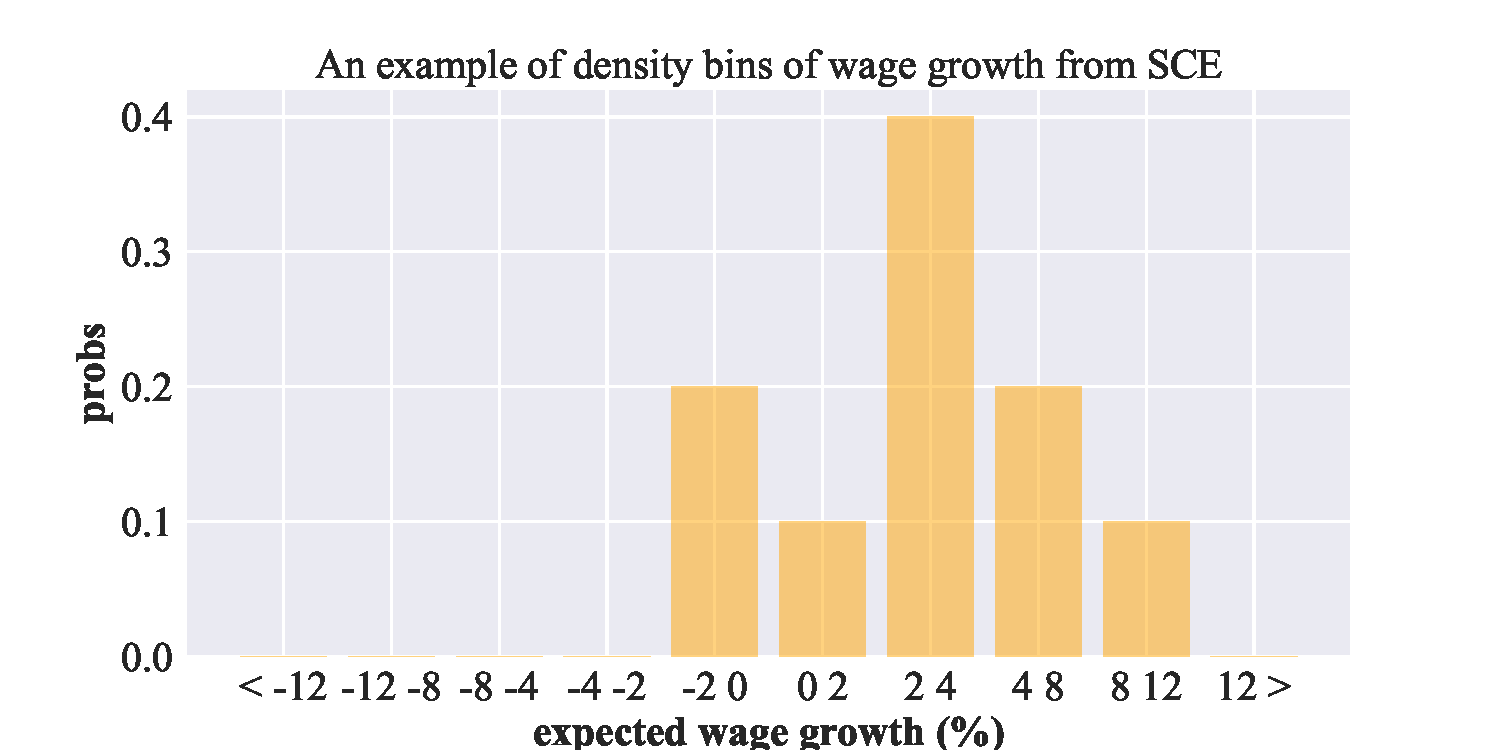
\includegraphics[width=0.7\textwidth]{figures/density_bin_example.pdf}
\end{figure}
\end{frame}



\begin{frame}{An illustration of the density forecast estimation}
	\begin{figure}
		\centering
		\label{fig: dens_est_illutration}
		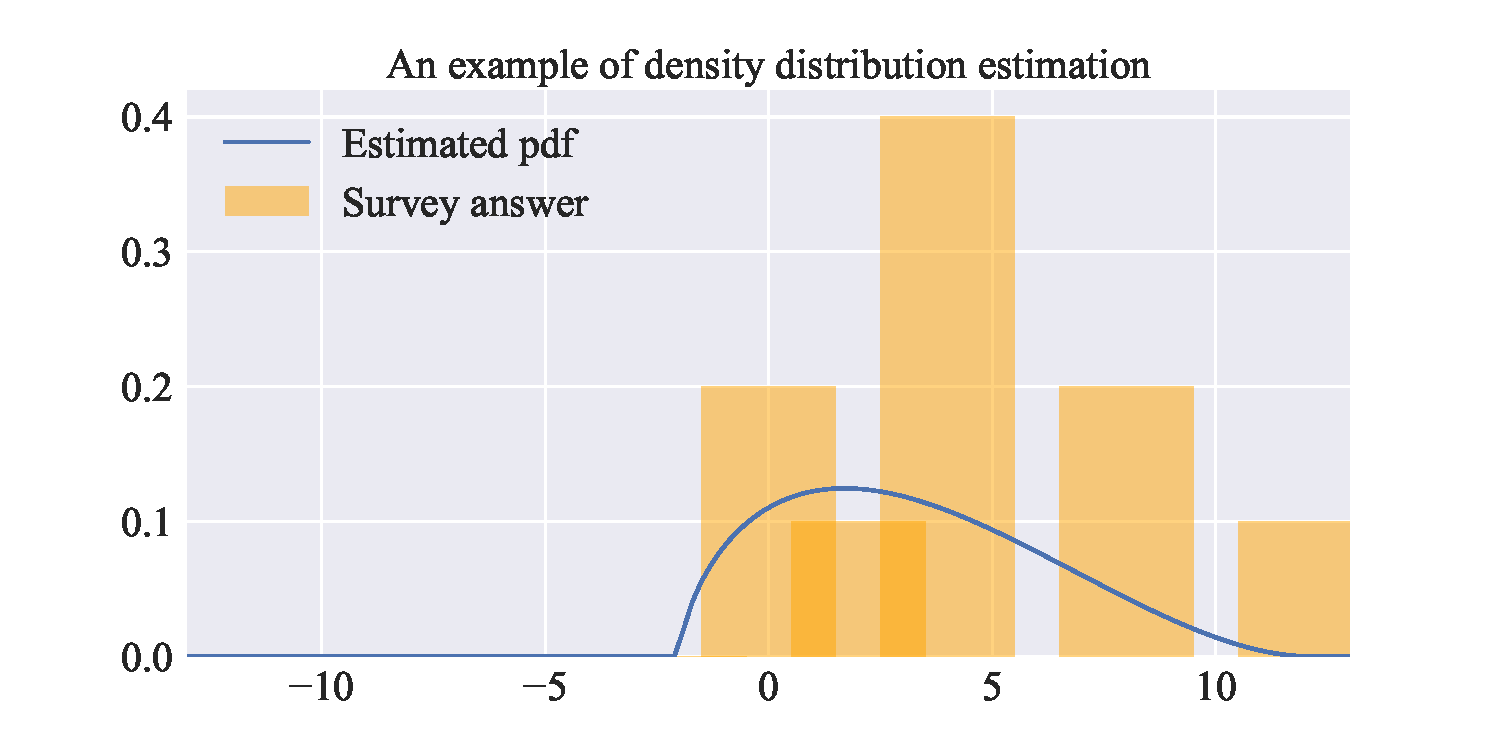
\includegraphics[width=0.6\textwidth]{figures/density_bin_est_example.pdf}
	\end{figure}
	
	\begin{itemize}
		\item  case 1. 3+ intervals with positive probs, a generalized beta dist
		\item case 2. exactly 2 adjacent intervals with positive probs: a triangle dist 
		\item case 3. one interval only: a uniform dist
	\end{itemize}
	
\end{frame}


\begin{frame}{Survey questions (continued)}
	\begin{itemize}
		\item Individual-specific bin-based forecast on $\Delta w_{i,t+1}$
		\begin{itemize}
			\item wage growth of the same job/position/hours
				\item exl. endogenous labor supply changes/promotion/demotion/separation 
				%\item Can be converted into the unconditional risk using perceived unemployment risk ( same-job-hour risk is just a lower bound).  %% I did not do the adjustment. I use same-job-hour income growth throughout my analysis.
		\end{itemize} 
		\item  Measurement of PR: 
		\begin{itemize}
			%\item expected growth, $\text{exp}_{i,t} = E_{i,t} (\Delta Y_{i,t+12})$
			\item variance: \textcolor{blue}{$\overline {Var}_{i,t}(\Delta w_{i,t+1})$}  
			\item computed from the density forecast
			% \item iqr: $\overline {iqr}_{i,t}(\Delta y_{i,t+12})$ 
			%\item skewness: $\overline {Skew}_{i,t}(\Delta y_{i,t+1})$
		\end{itemize}
		%\item nominal and real income growth 
		%\begin{itemize}
			%\item $\text{rexp}_{i,t} =E_{i,t}(\Delta y^r_{i,t+1}) =E_i(\Delta y_{i,t+1}^n) - E_{i,t+1}(\pi_{t+1})$
		%	\item $\overline{rvar}_{i,t}=\overline {var}_{i,t}(\Delta y_{i,t+1}^n) +  \overline {var}_{i,t}(\pi_{t+1})$
\item density estimation following \cite{engelberg_comparing_2009}			
\item restricted to attentive/high numeracy score sample
\item both nominal and real terms (adjusted by inflation uncertainty)
\end{itemize}
\end{frame}


\subsection{Framework}

\begin{frame}{Log wage process}
	\begin{equation*}
		\begin{split}
			\underbrace{w_{i,t}}_{\text{log wage}} = \underbrace{z_{i,t}}_{\text{predictable by the agent}}  + \underbrace{e_{i,t}}_{\text{stochastic component}}
		\end{split} 
	\end{equation*}
	
	\begin{itemize}
		\item individual \(i\) at time \(t\) 
		\item the time-series nature of $e_{i,t}$ to be specified later
	\end{itemize}
\end{frame}

\begin{frame}{Perceived risks (PR)}
	\begin{itemize}
		\item Wage growth 
		\begin{equation*}
			\begin{split}
				\Delta w_{i,t+1} & =\Delta z_{i,t+1} +\Delta e_{i,t+1} 
			\end{split}
		\end{equation*}
		\pause 
		\item \textcolor{blue}{To the agent: \textbf{conditional} variance under FIRE}
		\begin{equation*}
			\begin{split}
				%	Var^*_{i,t}(\Delta w_{i,t+1}) & =\sigma^2_{i,t+1|t}
				Var^*_{i,t}(\Delta w_{i,t+1}) & =Var^*_{i,t}(\Delta e_{i,t+1})
			\end{split}
		\end{equation*}
		\pause 
		% what we survey in the data is the conditional variance of the income  given information at time t. we assume agents have perfect information and correctly specify the model.  The information also  involves time -series nature of the shock also. 
		\item \textcolor{red}{To econometricians: \textbf{approximated unconditional} variance} 
		\begin{equation*}
			\begin{split}
				%	Var^c(\Delta \hat e_{i,c,t+1})     = \hat\sigma^2_{c,t}+ \hat\sigma^2_{c,t+1} - 2Cov^c(\hat e_{i,c,t},\hat e_{i,c,t+1})
				%Var^c(\hat e_{i,c,t+1})
				Var_c(\Delta \hat e_{i,c,t+1})     = 	Var_c(\Delta w_{i,t+1} - \Delta \hat z_{i,t+1} )
				%Var^c(\hat e_{i,c,t+1})
			\end{split}
		\end{equation*}
		\item $\hat e_{i,c,t+1}$: the first-step regression residual controlling observable vars
		\item group $c$: \textbf{assumed} to share income process/risks
		\begin{itemize}
			\item i.e. education/year of birth/gender/age
		\end{itemize}
		% when econometricians try to approximate, they first need to make sure predictable component is perfectly the same as the agents. given that, you want to further decompose this to refelct the exact time series nature of e. 
		
		%	\item \textcolor{blue}{To econometricians: \textbf{inequality} } 
		%		\begin{equation*}
			%		\begin{split}
				%		Var^c( \hat e_{i,c,t+1}) = \sigma^2_{c,t+1}
				%		\end{split}
			%	\end{equation*}
	\end{itemize}	
	%% therefore, I can examine how gross volatility estimated for each cohort is positively correlated with perceived risk from the data. 
	%% nice things about using gross volatility 
	%% not sensitive the stochastic nature of e
	%% not sensitive to the frequency of the data from PSID being annual or biennial 
\end{frame}



%\subsection{Permanent  versus transitory risks}


\begin{frame}{Time series structure of wage shocks}
	
	\begin{equation*}
		\begin{split}
			& e_{i,t} = \underbrace{p_{i,t}}_{\text{permanent}} + \underbrace{\theta_{i,t}}_{\text{ transitory}} \\
			& p_{i,t+1} = p_{i,t} + \psi_{i,t+1} \\
			& \psi_{i,t} \sim N(0,\sigma^2_{i,t,\psi}) \\
			& \theta_{i,t} \sim N(0,\sigma^2_{i,t,\theta}) \\
		\end{split} 
	\end{equation*}
\pause 
\begin{itemize}
	\item \textcolor{blue}{The agent's PR}
		\begin{equation*}
			Var^*_{i,t}(\Delta w_{i,t+1}) = \sigma^2_{i,t+1,\psi} + \sigma^2_{i,t+1,\theta}		\end{equation*}
\pause 
	\item \textcolor{red}{Econometricians' approximated PR}
\begin{equation*}
		\widehat {Var}_{c,t}(\Delta \hat e_{i,c,t+1})     =  \hat \sigma^2_{c,t+1,\psi} + \hat \sigma^2_{c,t+1,\theta} 
\end{equation*}
	\end{itemize}
\end{frame}



\begin{comment}
	\begin{frame}{Predictions from FIRE}
		
		\begin{itemize}
			\item  PR equal within groups with identical  risks 
			\begin{itemize}
				\item \textcolor{blue}{Question}: do similar people perceive similar degree of risks?
			\end{itemize}
			\item PR $\uparrow$ with income volatility
			\begin{itemize}
				\item \textcolor{blue}{Question}: do groups with higher volatility/inequality perceive higher risks?
				%\item the correlation depends on the time series nature of $e_{i,c,t}$ and $\sigma^2_{c}$
			\end{itemize}
			% $$Cov(Var^c(\hat e_{i,c,t}),Var^*_{i,c,t}(\Delta y_{i,c,t+1}))\approx 1$$
			\item PR independent from the income realization under state-independent risks
			\begin{itemize}
				\item \textcolor{blue}{Question} correlated with past/recent outcomes?
				%\item unless $\sigma^2_{e}$ is state dependent 
			\end{itemize} 
		\end{itemize} 
	\end{frame}
	
	\begin{frame}{Robustness to alternative considerations}
		
		\begin{itemize}
			\item superior information/unobserved heterogeneity
			\begin{itemize}
				\item higher income volatility/inequality due to omitted variable
			\end{itemize}
			\item measurement error in PR
			\begin{itemize}
				\item lower correlation but still positive
			\end{itemize}
			\item time aggregation
			\begin{itemize}
				\item higher frequency of income than observed series 
				%\item it matters once we assume time series property of $e$
			\end{itemize}
			\item time-varying/stochastic risks 
			\begin{itemize}
				\item a concern if realizations and perceptions not overlapping in time
				\item time-invariant risks for now: $\sigma^2_{c,t}=\sigma^2_{c} \quad \forall t$
			\end{itemize}
		\end{itemize} 
	\end{frame}
\end{comment}

\begin{frame}{Limitations with risk estimates from panel data}
	\begin{itemize}
		\item \textcolor{blue}{Superior information/unobservable heterogeneity}: $\hat z_{i,t} \neq z_{i,t}$ 
		\begin{itemize}
			\item $\hat z_{i,t}$ unlikely capture all in the information set of $i$ at $t$
			\begin{enumerate}
				\item Intrinsic heterogeneity of individual $i$ not observable by economists 
				\item Foresight about individual circumstance not available to economists
			\end{enumerate}
		\end{itemize}
		\pause
		\item \textcolor{blue}{Model misspecfication}
		\begin{itemize}
			\item Risks may differ within group $c$, but economists have to estimate it at the group level.
		\end{itemize}
		\pause
		\item \textcolor{red}{Surveyed PR} can be a better alternative 
		\begin{itemize}
			\item Directly conditional on information set of each $i$ at $t$
			\item No need to restrict risk heterogeneity by group $c$
			\item But need to be careful with measurement errors 
		\end{itemize}
	\end{itemize}	
\end{frame}


\subsection{Cross-sectional patterns}

%% add Low's estimates 


\begin{frame}{Survey PR $<$ Estimated PR within groups}
	\label{observable_heterogeneity_by_educ}
	\begin{figure}[ht]
		%\caption{Perceived Risk} 
		\label{compare_by_gender_educ}
		\centering
		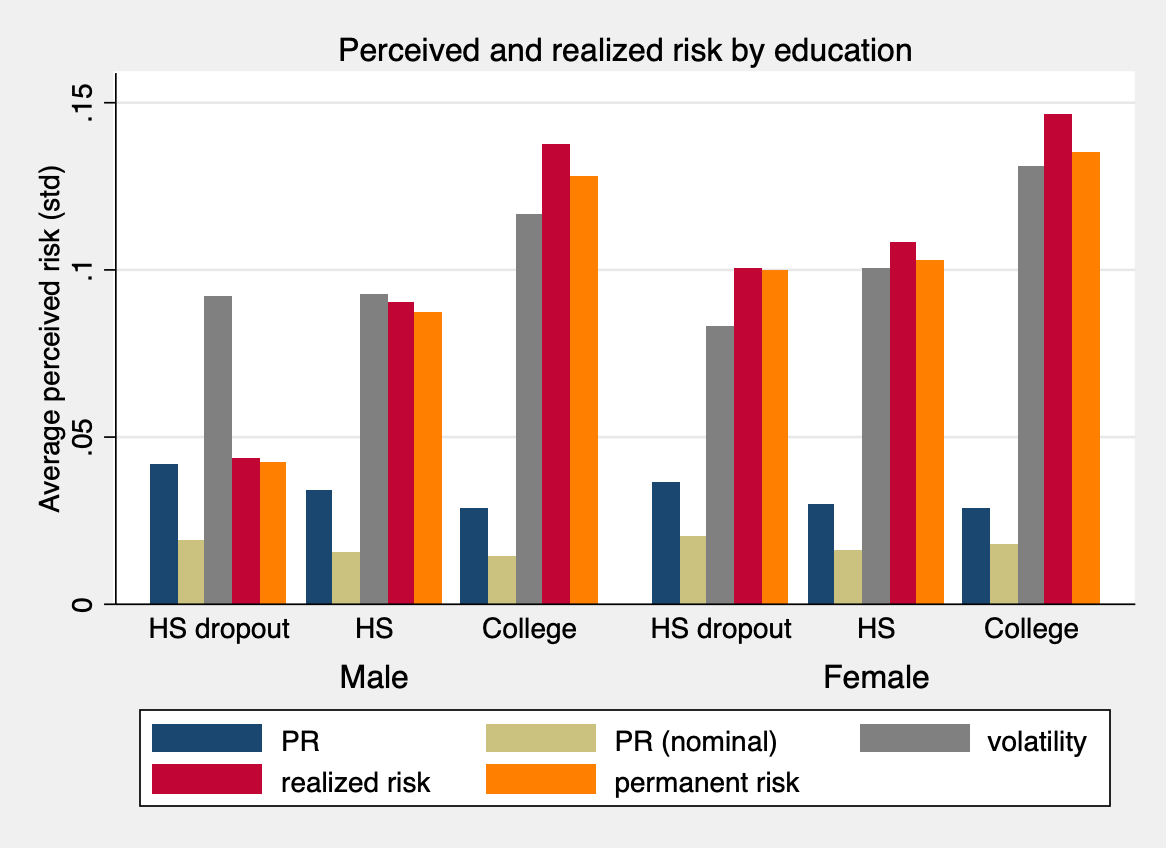
\includegraphics[width=0.60\textwidth]{figures/boxplot_rvar_compare_educ.png}
	\end{figure}
\pause 
	\begin{itemize}
		\item The wage risk estimates by  \cite{low2010wage}: 
		\begin{itemize}
			\item low education: permanent risk = 0.09, transitory risk = 0.08
			\item high education: permanent risk = 0.106, transitory risk = 0.08
	\end{itemize}
\end{itemize}
	%\hyperlink{monthly_decomposition_compare}{\beamerbutton{Back}} 
\end{frame}

\begin{frame}{Survey PR $<$ Estimated PR within groups, continued}
	\label{observable_heterogeneity_by_age}
	\begin{figure}[ht]
		%\caption{Perceived Risk} 
		\label{compare_by_gender_age}
		\centering
		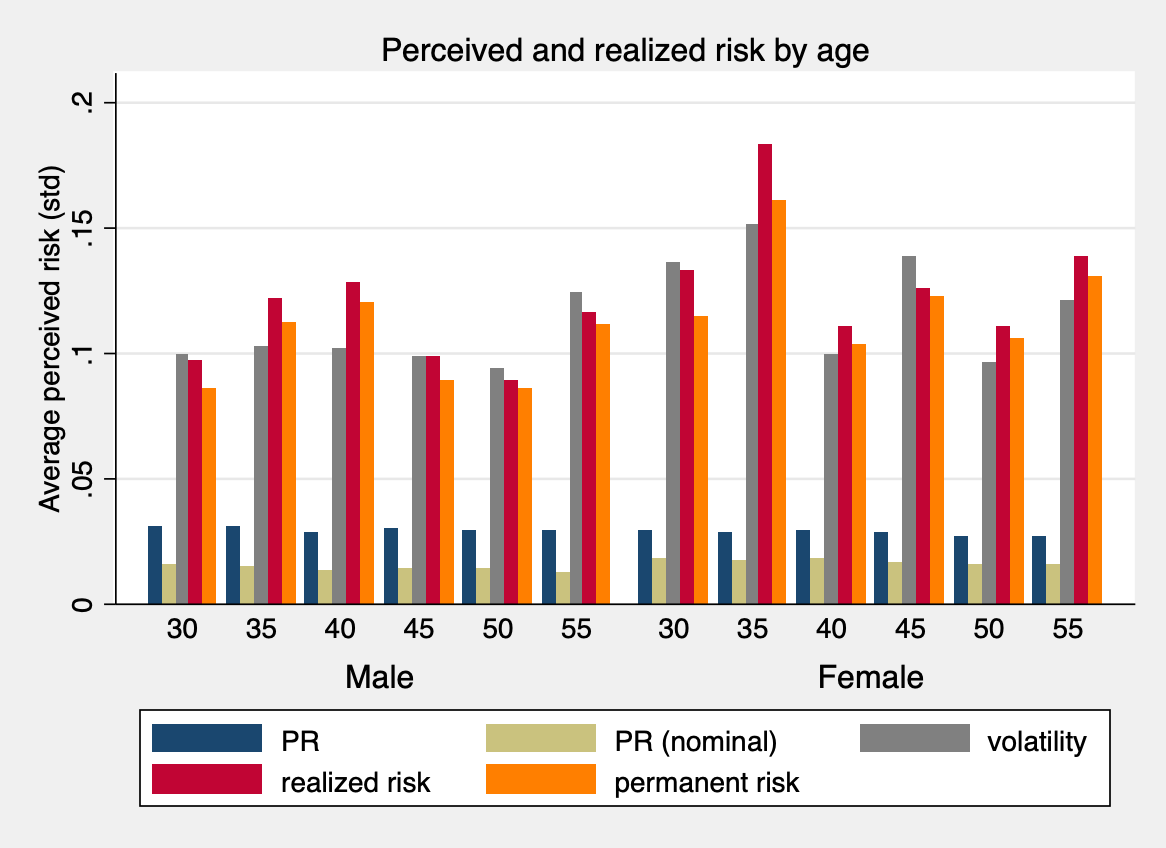
\includegraphics[width=0.70\textwidth]{figures/boxplot_rvar_compare_age.png}
	\end{figure}
	%\hyperlink{monthly_decomposition_compare}{\beamerbutton{Back}} 
\end{frame}


\begin{frame}{Unobservable heterogeneity}
	\begin{figure}
		\centering
		\label{rincstd_hist}
			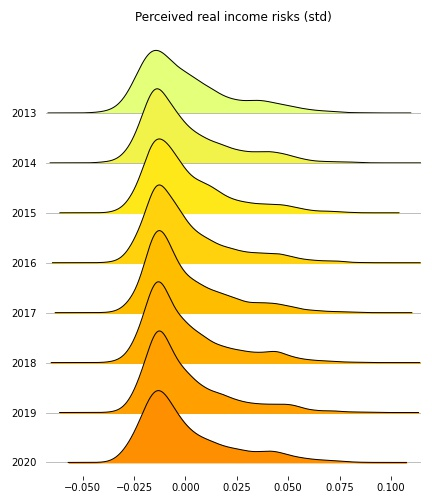
\includegraphics[width=0.4\textwidth]{figures/joy_rincstd.jpg}
	\end{figure}
	\begin{itemize}
		\item  PR residuals controlling for observables $+$ time FE ($R^2=0.10$) 
		\item average PR:  $3.5\%$ in std; 10/90 IQR: $5.2\%$ in std \quad \hyperlink{appendix:incstd}{\beamerbutton{nominal}}  
	\end{itemize}
\end{frame}


\begin{frame}{Permanent versus transitory risks}
	\label{monthly_decomposition_compare}
	\begin{figure}[ht]
		\centering
		\begin{subfigure}[b]{0.32\textwidth}
			\caption{permanent}
			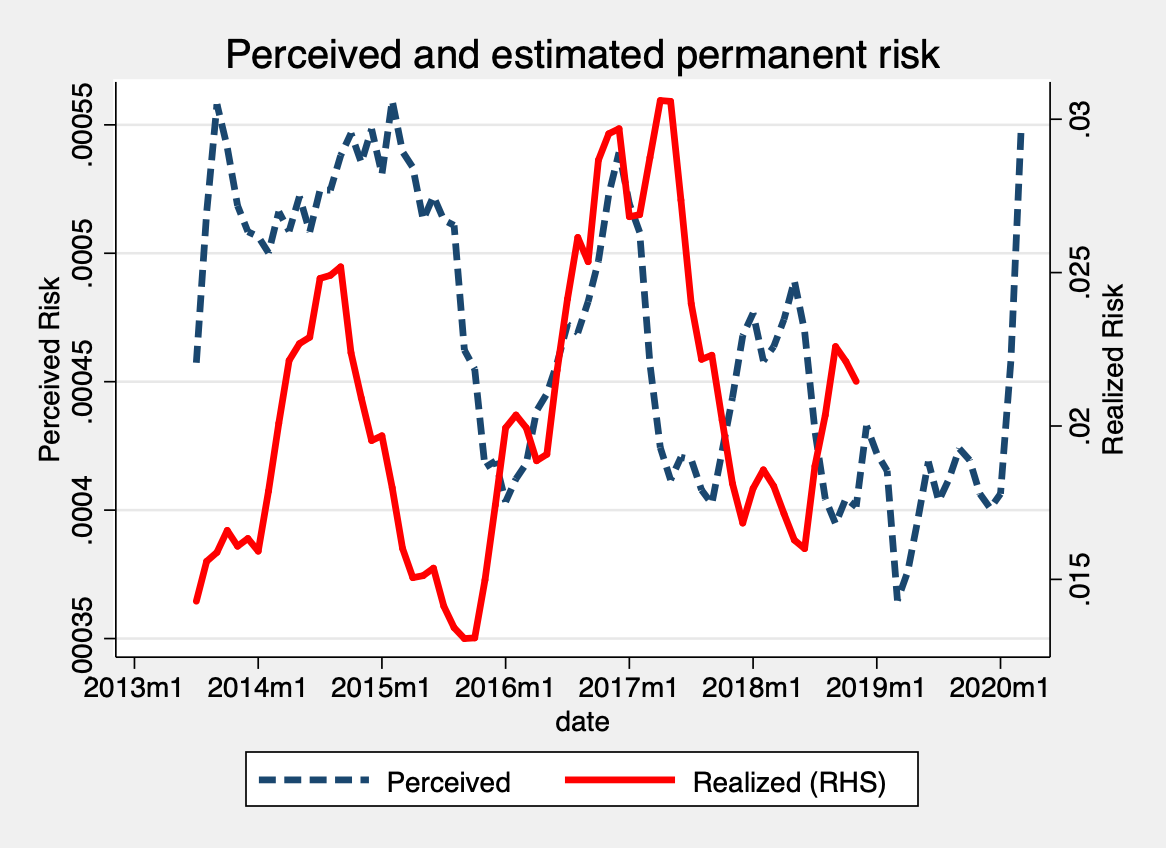
\includegraphics[width=\textwidth]{figures/real_permanent_compare.png}
		\end{subfigure}
		\begin{subfigure}[b]{0.32\textwidth}
			\caption{transitory}
			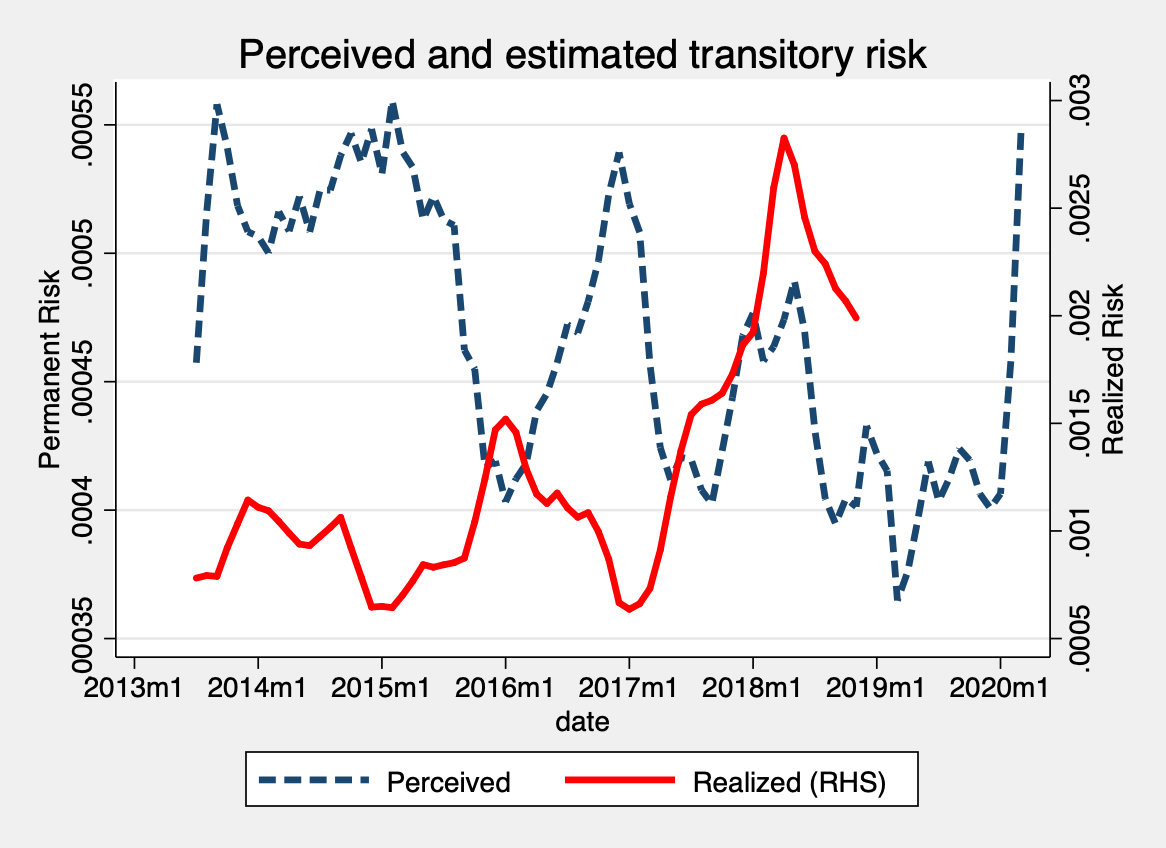
\includegraphics[width=\textwidth]{figures/real_transitory_compare.png}
		\end{subfigure} 
		\begin{subfigure}[b]{0.32\textwidth}
		\caption{volatility}
		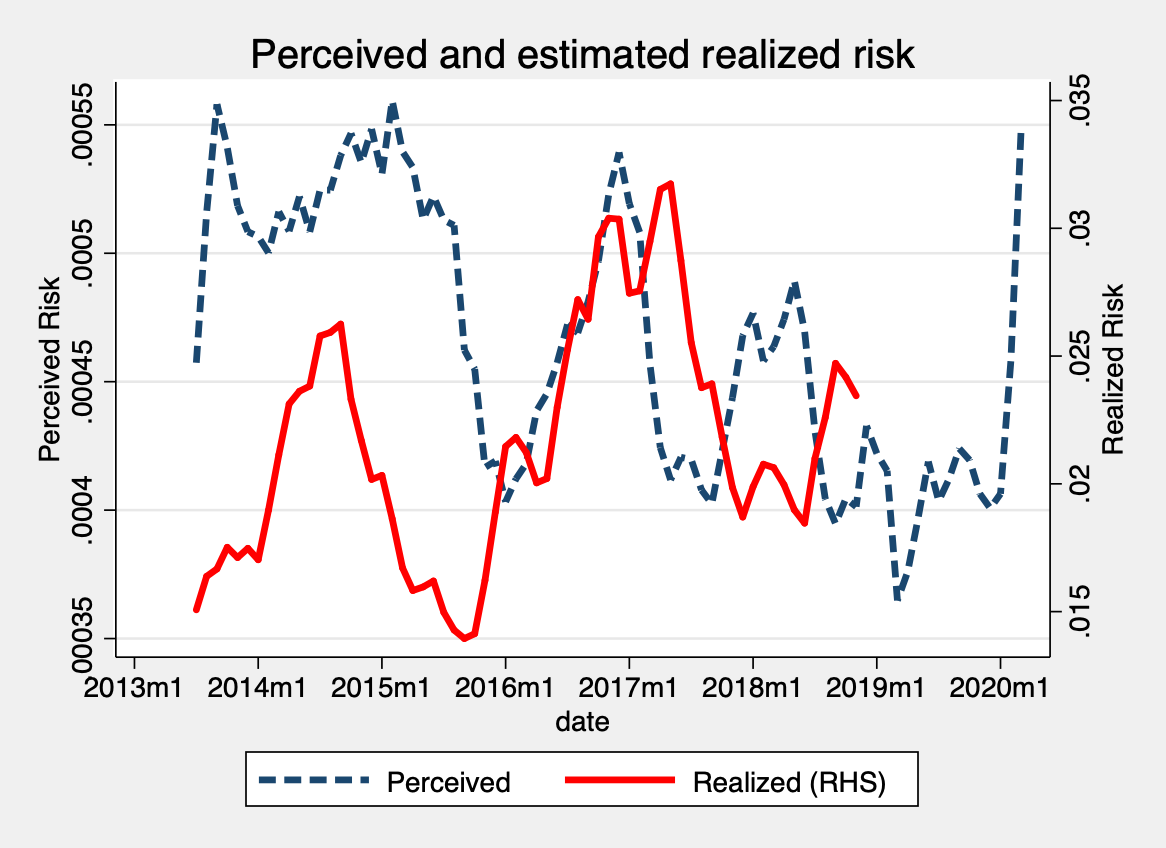
\includegraphics[width=\textwidth]{figures/real_volatility_compare.png}
	\end{subfigure} 
	\end{figure}
	\begin{itemize}
		\item i.e. one-year-ahead perceived risk at 2014m1 v.s. realized risk over the same period
		\item wage rate for the same job/hours/position
		\item estimated monthly risks aggregated into annual frequency 
	\end{itemize}
\hyperlink{appendix:monthly_inequality_vol}{\beamerbutton{More details}} 
\end{frame}



\begin{comment}
\begin{frame}{Perceptions versus economists' estimates}
	
	
	\begin{table}
		\centering
		%\caption{Estimated realized income risk and perceptions}
		\label{risk_compare}
		\adjustbox{max height=0.4\textheight, max width=\textwidth}{ 
		\begin{tabular}{lllllll}
			\hline \hline 
			& PR(mean)   & PR(median) & Volatility & RealizedRisk & PRisk & TRisk  \\
			\hline 
			gender                 &            &            &                    &              &       &        \\
			\hline 
			1 (50\%)               & 0.03       & 0.022      & 0.105              & 0.115        & 0.109 & 0.0238 \\
			2 (49\%)               & 0.028      & 0.022      & 0.118              & 0.131        & 0.122 & 0.0322 \\
			&            &            &                    &              &       &        \\
			\hline 
			\multicolumn{2}{l}{education group} &            &                    &              &       &        \\
			\hline 
			HS dropout (0\%)       & 0.036      & 0.022      & 0.088              & 0.071        & 0.07  & 0.0063 \\
			HS graduate (42\%)     & 0.03       & 0.022      & 0.096              & 0.098        & 0.094 & 0.0176 \\
			College/above (56\%)   & 0.028      & 0.021      & 0.124              & 0.142        & 0.132 & 0.0357 \\
			&            &            &                    &              &       &        \\
			\hline 
			5-year age             &            &            &                    &              &       &        \\
			\hline 
			20 (2\%)               & 0.037      & 0.031      & 0.094              & 0.069        & 0.068 & 0.0061 \\
			25 (12\%)              & 0.032      & 0.027      & 0.111              & 0.157        & 0.156 & 0.0083 \\
			30 (12\%)              & 0.03       & 0.023      & 0.116              & 0.112        & 0.098 & 0.0372 \\
			35 (13\%)              & 0.029      & 0.021      & 0.125              & 0.149        & 0.134 & 0.0524 \\
			40 (13\%)              & 0.028      & 0.02       & 0.1                & 0.119        & 0.111 & 0.0287 \\
			45 (14\%)              & 0.028      & 0.02       & 0.119              & 0.113        & 0.106 & 0.0224 \\
			50 (15\%)              & 0.027      & 0.019      & 0.095              & 0.1          & 0.096 & 0.0203 \\
			55 (15\%)              & 0.027      & 0.018      & 0.122              & 0.128        & 0.121 & 0.0283 \\
			\hline 
			Full sample (100\%)          & 0.029      & 0.021      & 0.112              & 0.123        & 0.115 & 0.0279 \\
			\hline \hline 
		\end{tabular}
		}
	\end{table}
\end{frame}
\end{comment}



\subsection{Unemployment risks}
% this goes back to main slides for longer presentation 
%\subsection{Perceived unemployed risks}
\begin{frame}{Perceived UE risks and realization}
	\begin{figure}
		\centering
		\label{ue_expectations}
		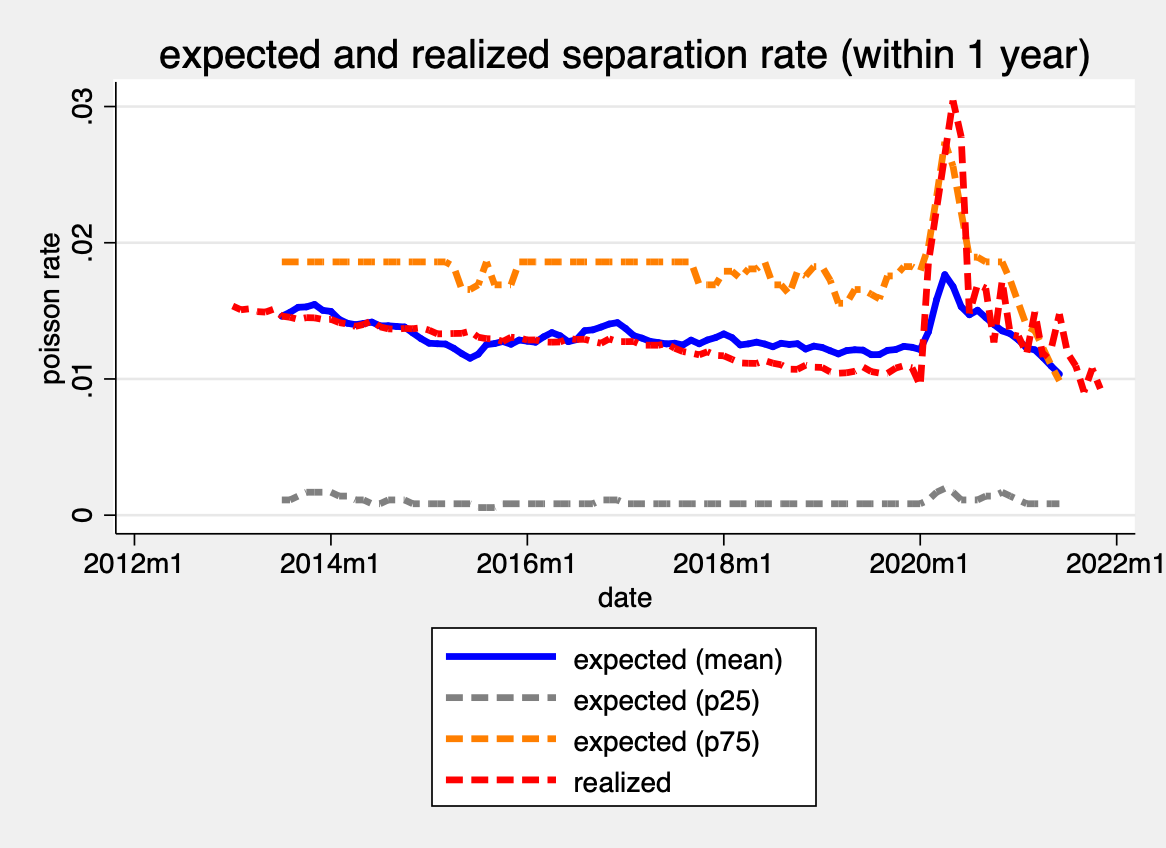
\includegraphics[width=0.45\textwidth]{figures/separation_rate_1y.png} 
		\hfill
		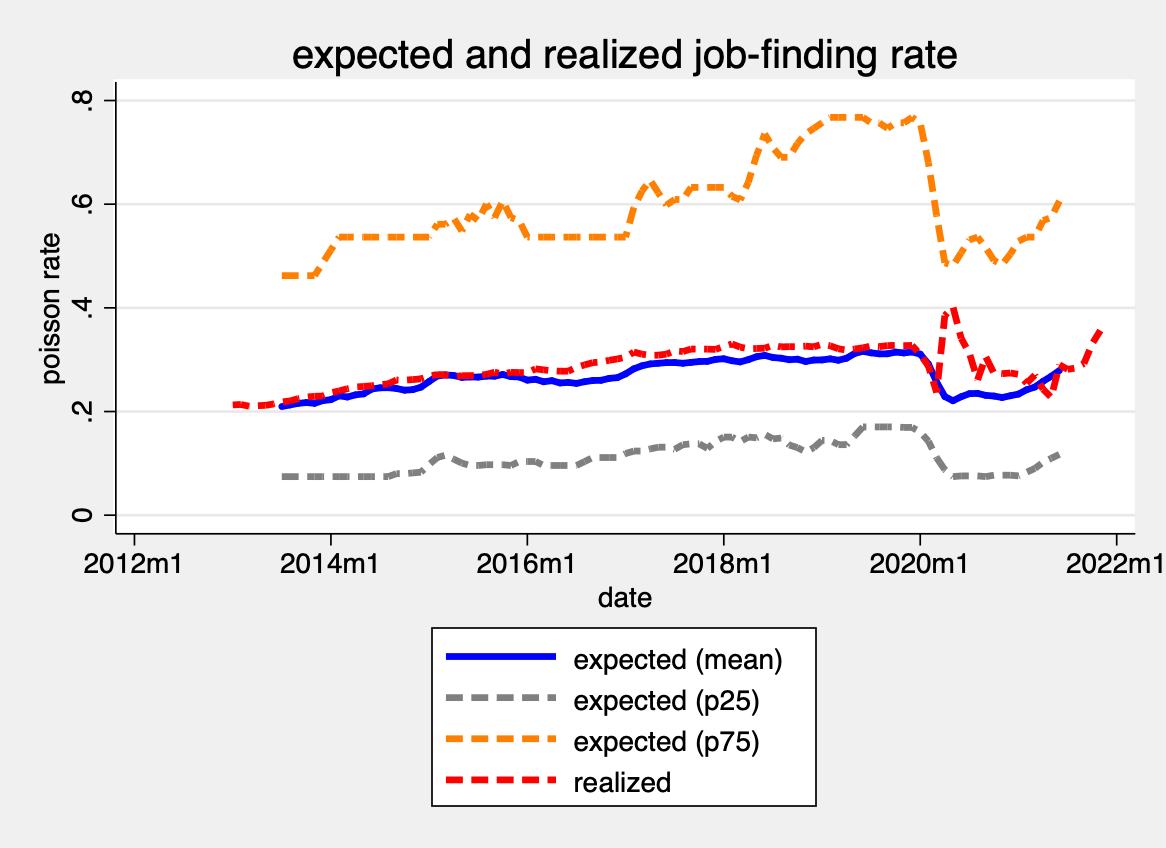
\includegraphics[width=0.45\textwidth]{figures/job_finding_rate.png} 
	\end{figure}
	\begin{itemize}
		\item the realization computed from CPS panel data of workers following \cite{fujita2009cyclicality}
	\end{itemize}
\end{frame}


\subsection{Perceived risks and decisions}


\begin{frame}{Perceived risks and household spending}
	
	\begin{eqnarray*}
		E_{i,t} (\Delta c_{i,t+1}) = u_0 + \textcolor{red}{u_1} \text{Var}_{i,t} (\Delta w_{i,t+1}) + \xi_{i,t}  
	\end{eqnarray*}
	\begin{table}
		\centering
		%\caption{Perceived income risks and household spending}
		\label{spending_reg}
		\adjustbox{max height=0.5\textheight, max width=\textwidth}{ 
			
\begin{tabular}{lllllll}
	\hline 
	& (1)      & (2)      & (3)      & (4)      & (5)      & (6)      \\
		\hline 
	perceived earning risk           & 8.394*** & 8.399*** & 3.642*** & 3.243*** &          &          \\
	& (1.175)  & (1.176)  & (0.533)  & (0.537)  &          &          \\
	&          &          &          &          &          &          \\
	perceived earning risk (nominal) &          &          &          &          & 3.656*** &          \\
	&          &          &          &          & (0.990)  &          \\
	&          &          &          &          &          &          \\
	perceived ue risk                &          &          &          &          &          & 0.353*** \\
	&          &          &          &          &          & (0.0553) \\
		\hline 
	R-squared                        & 0.0010 & 0.00282  & 0.928    & 0.928    & 0.941    & 0.633    \\
	Sample Size                      & 53178    & 53178    & 53178    & 53178    & 54584    & 6269     \\
	Time FE                          & No       & Yes      & No       & Yes      & Yes      & No       \\
	Individual FE                    & No       & No       & Yes      & Yes      & Yes      & Yes     \\
		\hline 
\end{tabular}
		}
	\end{table}
	\begin{itemize}
		\item  Higher perceived risks $\rightarrow$ higher expected spending growth. 
	\end{itemize}
\end{frame}


\begin{frame}{Calibrating heterogenous PRs from SCE survey}
	\label{calibration_survey_risks}
	
	\begin{itemize}
		\item Fit a truncated log-normal dist over the cross-section of PRs 
		\item Uncover unobserved heterogeneity in wage growth using the difference between reported PR and the estimated PR. 
	\end{itemize}
	
	\begin{figure}
		\centering
		\label{fig:calibration_survey}
		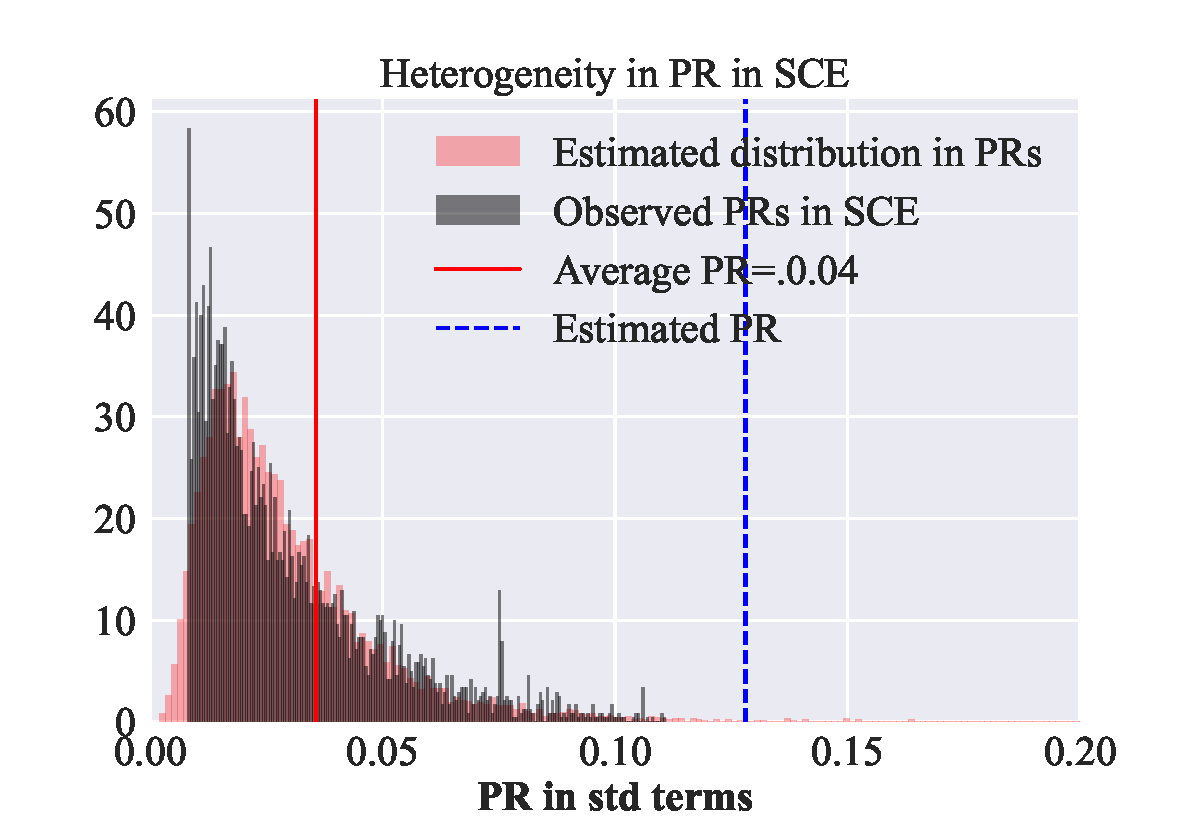
\includegraphics[width=0.35\textwidth]{figures/log_normal_pr_fit.pdf} 
		\pause
		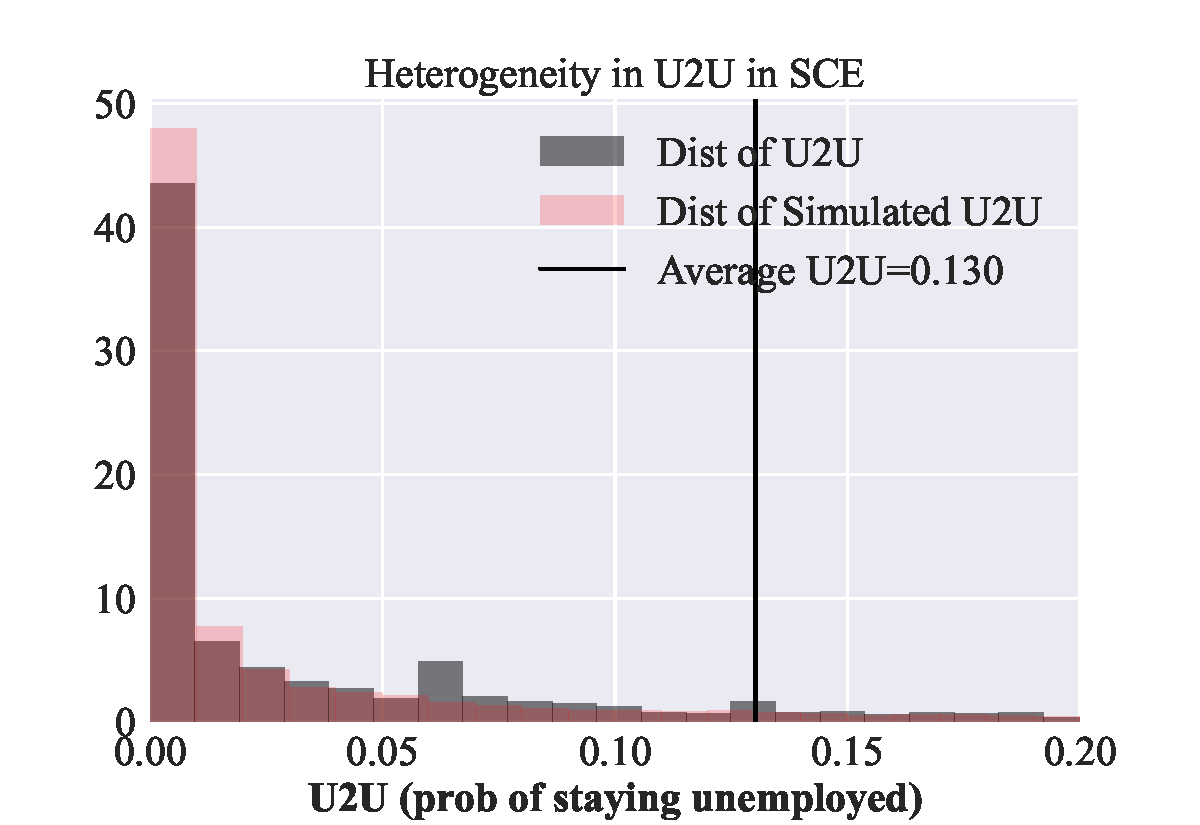
\includegraphics[width=0.35\textwidth]{figures/log_normal_u2u_fit.pdf} 
		\\
		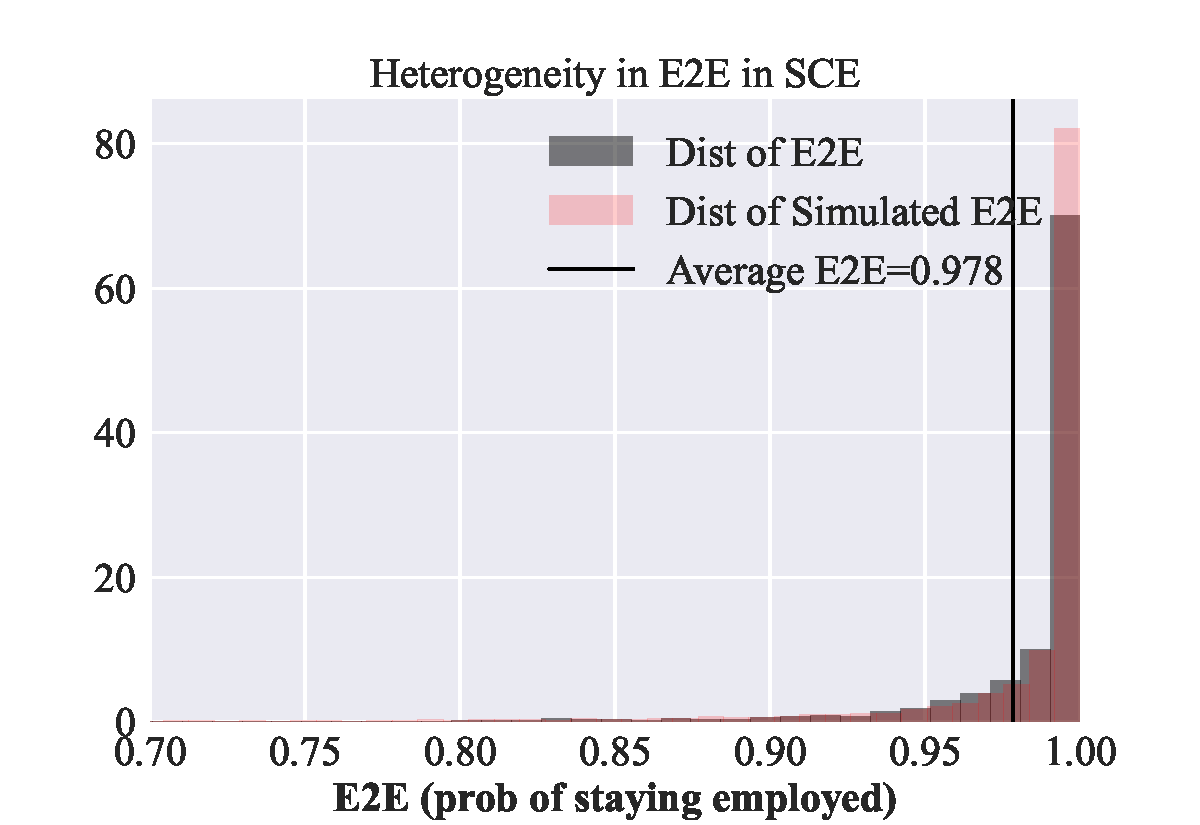
\includegraphics[width=0.35\textwidth]{figures/log_normal_e2e_fit.pdf} 
		\pause
		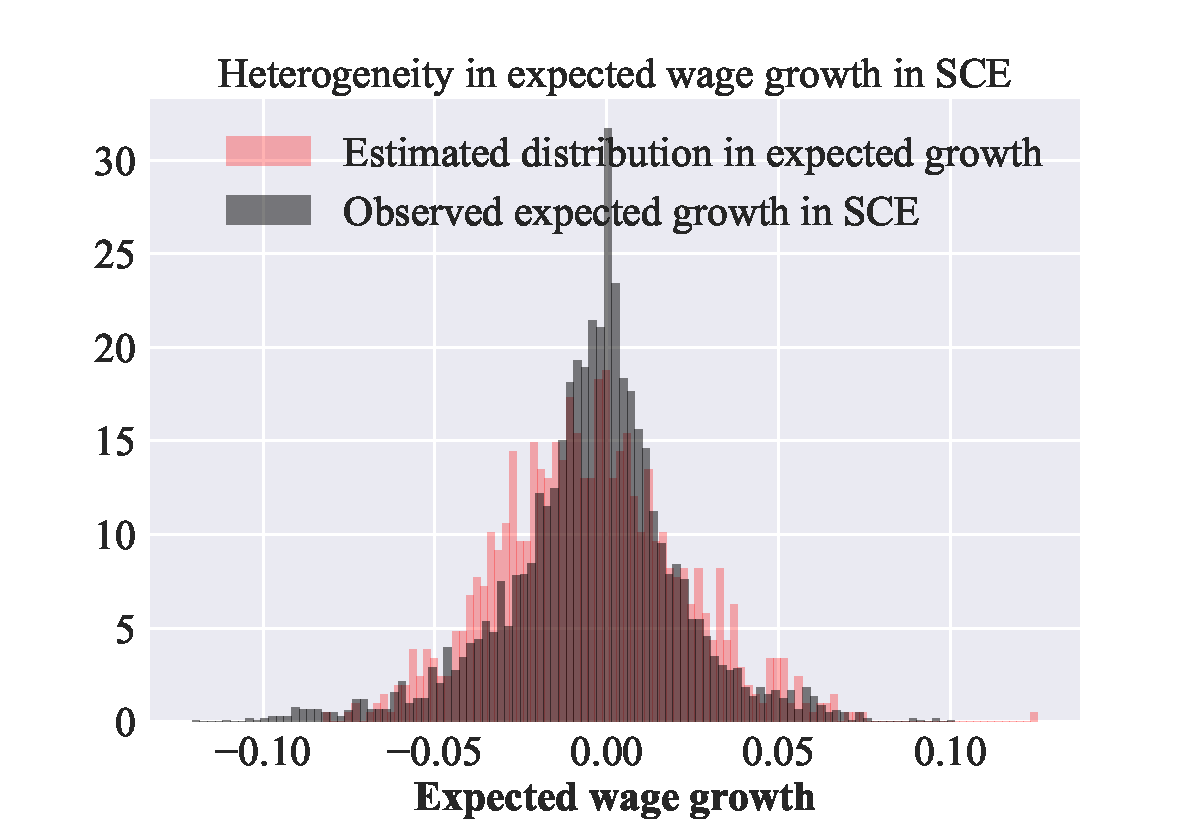
\includegraphics[width=0.35\textwidth]{figures/log_normal_exp_fit.pdf} 
	\end{figure}
	
\end{frame}


\begin{comment}

\subsection{Summary of empirical findings}
\begin{frame}{Taking stock}
	
	\begin{itemize}
		\item Observable heterogeneity 
		\begin{itemize}
			\item  some is consistent with inter-group differences as commonly assumed 
		%	\item other covariates 
	%		\begin{itemize}
	%			\item $\downarrow$ with education, household income, being a male
	%			\item $\uparrow$  with numeracy score, self-employed job, perceived individual UE risks, aggregate UE expectations, experienced volatility 
	%		\end{itemize}
		\end{itemize}
		\pause
		\item But huge amount of \textcolor{blue}{unobservable} heterogeneity remains
		\begin{itemize}
			\item including all above: $R^2 =0.10$
			\item individual fixed effects only: $R^2=0.71$
		\end{itemize}
		\pause
		\item Why not directly use survey-reported PR?
		\begin{itemize}
			\item a resolution to ``superior information''/ unobserved heterogeneity
			\item heterogeneity in wage risks without grouping people
		\end{itemize}
	\pause 
	\item But need to be careful with 
	\begin{itemize}
		\item measurement errors in survey 
		\item behavioral bias. 
	\end{itemize} 
	\end{itemize} 
\end{frame}

\end{comment}

\begin{comment}
	
\begin{frame}{A simple model of risk perception}
	\label{model}
	\begin{itemize}
		\item Under FIRE 
		\begin{equation*}
			\begin{split}
				&{ Var}^*_{i,c,t}(\Delta y_{i,c,t}) =  \sigma^2_{\psi,c} + \sigma^2_{\epsilon,c} 
			\end{split}
		\end{equation*}
		\item  Under imperfect understanding
		\begin{itemize}
			\item $\phi$ and $\sigma^2_{\epsilon,c}$ are not perfectly known 
			\item all realized shocks are perfectly observed  
		\end{itemize}
	\end{itemize}
	\begin{equation*}
		\begin{split}
			& \widetilde{ Var}_{i,c,t}(\Delta y_{i,c,t+1}) =  \sigma^2_{\psi,c} + \tilde \sigma^2_{\epsilon,c,t} \\
			&\textcolor{blue}{\text{Experience-dependence: }}	\tilde \sigma^2_{\epsilon,c,t} =  \frac{\overbrace{Var_{i,c,t}(\eta_{i,c,t})}^{\text{experienced volatility}} }{1+\tilde \phi^2_{i,c,t}} \\
			&\textcolor{blue}{\text{State-dependence: }}		\tilde \phi_{i,c,t} =  \delta(\epsilon_{i,c,t})  
		\end{split}
	\end{equation*}
\end{frame}

\end{comment}



\section{Model}

\begin{frame}{Model overview}
	\begin{itemize}
		\item Overlapping generation 
		\item General equilibrium 

		\item Uninsured idiosyncratic income risks
		\begin{itemize}
		\item Permanent+ transitory idiosyncratic wage shock
		\item Persistent unemployment spells
		\end{itemize}
	\item No aggregate risk a la \cite{krusell1998income} 
		\item A blend of \cite{huggett1996wealth} and \cite{carroll1997buffer}
		\item Only one risk-free asset 
	\item Calibrating income risks \textcolor{red}{using survey} versus \textcolor{blue}{estimates from panel} 
	\item Extension: subjective risk perceptions 
	\begin{itemize}
		\item Individuals swing between low/high risk perceptions
	\end{itemize}

	\end{itemize}
\end{frame}


\begin{frame}{Preview of the model mechanisms}
	\begin{itemize}
		\item On \textcolor{red}{level} of savings
		\begin{enumerate}
			\item $\downarrow$ \textcolor{blue}{lower PR}: lower precautionary saving motives $\rightarrow$ less liquid holding $\rightarrow$ higher MPC
			%\item $\uparrow$  \textcolor{blue}{state-dependence}: a mean-preserving spread in risks $\rightarrow$  more precautionary savings \cite{caballero1990consumption}
			%	 	\pause
			%\item $\uparrow$ \textcolor{blue}{extrapolation}: lower income/unemployment $\rightarrow$ higher PR $\rightarrow$ intensified precautionary motive 
			%	\pause
			%	\item $\uparrow$ \textcolor{blue}{counter-cyclical risks}:  amplified business cycle fluctuations \cite{bayer2019precautionary}
		\end{enumerate}
	\pause
		\item On \textcolor{red}{wealth inequality}
		\begin{itemize}
			\item 	$\uparrow$ \textcolor{blue}{heterogeneous PR} $\rightarrow$ heterogeneity in saving/wealth
			%\item $\uparrow$ Indirect effect: \textcolor{blue}{lower PR} $\rightarrow$ lower self-insurance $\rightarrow$ higher  ex-post wealth inequality
		\end{itemize}
	\end{itemize}
\end{frame}


\begin{frame}{Benchmark model}

\begin{equation*}
	\textrm{max}\quad  \mathbb{E}\left[\sum^{\tau=L-1}_{\tau=0}(1-D)^\tau\beta^\tau u(c_{i,\tau})\right] 
\end{equation*}



\begin{equation*}
	\begin{split}
		& \underbrace{a_{i,\tau}}_{\text{Savings}} = \underbrace{m_{i,\tau}}_{\text{Cash in hand}} - c_{i,\tau} \\
		& b_{i,\tau+1} = a_{i,\tau} R  \\
		& m_{i,\tau+1}   = b_{i,\tau+1}+(1-\underbrace{\lambda}_{\text{Income tax}})(1-\underbrace{\lambda_{SS}}_{\text{SS tax}})y_{i,\tau+1}\\
		& a_{i,\tau} \geq 0 
	\end{split}
\end{equation*}


\begin{itemize}
	\item CRRA: $u(c) = \frac{c^{1-\rho}}{1-\rho}$
	\item Work age: $\tau=1, 2...,T$ (since entering job market) 
	\item Life length: $\tau=1, 2...,L$  (since entering job market)
	\item Survival probability: 1-D
\end{itemize}

\end{frame}



\begin{frame}{Income process over the life-cycle}
	\begin{itemize}
		\item income
	\begin{equation*}
		\begin{split}
			y_{i,\tau} = n_{i,\tau}W  \\
			n_{i,\tau} = p_{i,\tau}\xi_{i,\tau}
		\end{split}
	\end{equation*}
	\item permanent component 
\begin{equation*}
	\begin{split}
		p_{i,\tau} = G_\tau p_{i,\tau-1}\psi_{i,\tau}, \quad
		log (\psi_{i,\tau}) \sim N(-\sigma^2_{\psi}/2,\textcolor{red}{\sigma^2_{\psi}}) \quad \forall \tau \leq T \\
	\end{split}
\end{equation*}
	\item persistent/transitory component 
\begin{equation*}
	\begin{split}
\xi_{i,\tau} =   \left\{
\begin{array}{ll}
	\theta_{i,\tau} \quad \text{if} \quad \nu_{i,\tau} =e \quad \& \quad  \tau \leq T, \quad log(\theta_{i,\tau}) \sim N(-\frac{\sigma^2_\theta}{2},\textcolor{red}{\sigma^2_\theta})\\
	\zeta \quad \text{if} \quad \nu_{i,\tau} = u \quad \& \quad \tau \leq T  \\
	\mathbb{S} \quad \text{if}  \quad \tau > T
\end{array} \right. 
\end{split}
\end{equation*}
	\item transition probability between $\nu=u$ and $\nu=e$
\begin{equation*}
	\pi (\nu_{\tau+1}|\nu_{\tau})= 
	\begin{bmatrix} 
		\textcolor{red}{\mho} & 1-\mho  \\
		1-E & \textcolor{red}{E}
	\end{bmatrix}
	\quad
\end{equation*}
	\end{itemize}
\end{frame}


\begin{frame}{Macroeconomic environment}
	\begin{itemize}
		\item \textcolor{blue}{Technology}
		\begin{equation*}
			Y = Z K^{\alpha}N^{1-\alpha}
		\end{equation*}
	\pause
		\item \textcolor{blue}{Government (balance budget)}
	\begin{equation*}
		\begin{split}
		\label{Eq:gov}
	&	\lambda \left[ 1-\Pi^\mho  + \zeta \Pi^\mho \right]  = \zeta \Pi^\mho    \\
	&	   \lambda_{SS} \sum^{T}_{\tau=1}G_{\tau}(1-\Pi^\mho) = \mathbb{S} \sum^{L}_{\tau=T+1} G_{\tau} 
	   \end{split}
	\end{equation*}
	
	\pause
		\item \textcolor{blue}{Demographics}
		\begin{itemize}
			\item Stable age distribution  $\{\mu_\tau \}_{\mu=1,2,..L}$ 
			\begin{equation*}
			 \mu_{\tau+1} = (1-D)\mu_{\tau}, \quad \sum^{L}_{\tau=1}\mu_{\tau} = 1
			\end{equation*}
		\end{itemize}
	\pause
		\item \textcolor{blue}{Zero or positive accidental bequests}:  lum-sum of a fraction of the deceased' wealth
	%	 \begin{itemize}
		% 	\item Newborn starts with a bank-balance equal to $0-1$ fraction of the lump-sum of the accidental deceased's wealth 
%		 \end{itemize}
	\end{itemize}
\end{frame}


\begin{frame}{Value function and transitions}
	\begin{itemize}
		\item Value function
		\begin{equation*}
			\begin{split}
				V_{\tau}(\underbrace{\nu_{i,\tau}, m_{i,\tau}, p_{i,\tau}}_{x_{i,\tau}})  =  & \underset{\{c_{i,\tau},a_{i,\tau}\}}{\textrm{max}} \quad   u(c_{i,\tau}) \\
		& +  (1-D)\beta \mathbb{E}_{\tau}\left[V_{\tau+1}((\nu_{i,\tau},m_{i,\tau+1}, p_{i,\tau+1})\right] 
			\end{split}
		\end{equation*}
	
	\item Transitions
		\begin{equation*}
		\label{Eq:DistDyn}
		\psi_{\tau}(B)=\int_{x \in X} \underbrace{P(x, \tau-1, B)}_{\text{transition funcs}}  \mathrm{d}\psi_{\tau-1} \quad \text { for all } \quad B\in B(X)
	\end{equation*}
	
	\end{itemize}
\end{frame}


\begin{frame}{Stationary equilibrium (StE)}
\begin{itemize}
	\item Optimal consumption and saving policies given $W$, $R$, $\lambda$
	\item Distribution evolution consistent with optimal $c$ and $a$ policies and income risks
	\item The factor markets clear 
	\begin{equation*}
	\begin{split}
		& \sum_{\tau} \mu_{\tau} \int_{X}a(x, \tau) \mathrm{d} \psi_{\tau}=K \\
		& \sum^{T-1}_{\tau=0} \mu_{\tau} \Pi^E_\tau= N
	\end{split}
	\end{equation*}
\item Firm optimization under competitive factor markets.
$$W = Z(1-\alpha) (K/N)^\alpha $$
$$R = 1+Z\alpha (K/N)^{\alpha-1} - \delta$$
%\item Newborn's bank balance equal to accidental bequests
\item Balanced government budget 
\end{itemize}
\end{frame}


\begin{frame}{Calibration of the benchmark model}
	\label{appendix:calibration}	
	\begin{table}[p]
		\centering
		\caption{Model parameters}
		\label{tab:calibration}
		\begin{adjustbox}{width={0.8\textwidth}}
			\begin{tabular}{llll}
				\hline 
				
				block             & parameter name              & values & source                               \\
				\hline 
				
				risk              & $\sigma_\psi$               & 0.15   & Median estimates from the literature \\
				risk              & $\sigma_\theta$             & 0.15    & Median estimates from the literature \\
				risk              & $U2U$                       & 0.18   & Median estimates from the literature \\
				risk              & $E2E$                       & 0.96   & Median estimates from the literature \\
				\hline 
				
				initial condition & $\sigma_\psi^{\text{init}}$ & 0.629  & Estimated for age 25 in the 2016 SCF \\
				initial condition & bequest ratio               & 0      & assumption                           \\
				\hline 
				
				life cycle        & $T$                         & 40     & standard assumption                  \\
				life cycle        & $L$                         & 60     & standard assumption                  \\
				life cycle        & $1-D$                       & 0.994  & standard assumption                  \\
				\hline 
				
				preference        & $\rho$                      & 1      & standard assumption                  \\
				preference        & $\beta$                     & 0.98   & standard assumption                  \\
				\hline 
				
				policy            & $\mathbb{S}$                & 0.65   & U.S. average                         \\
				policy            & $\lambda$                   & 0      & endogenously determined              \\
				policy            & $\lambda_{SS}$              & 0      & endogenously determined              \\
				policy            & $\mu$                       & 0.15   & U.S. average                         \\
				\hline 
				production        & $W$                         & 1      & target values in steady state        \\
				production        & K2Y ratio                   & 3      & target values in steady state        \\
				production        & $\alpha$                    & 0.33   & standard assumption                  \\
				production        & $\delta$                    & 0.025  & standard assumption          \\
				\hline 
			\end{tabular} 
		\end{adjustbox}
	\end{table}
	\hyperlink{StE_dist_compare}{\beamerbutton{Back}} 
\end{frame}

\begin{frame}{Deterministic wage profile over life cycle}
	\begin{figure}[!ht]
	\begin{center}
		\adjustimage{max size={0.8\linewidth}{0.8\paperheight}}{figures/age_wage_profile.pdf}
	\end{center}
\end{figure}
\begin{itemize}
\item 	{\scriptsize Estimated from SIPP with a fourth-order age polynomial regression}
\end{itemize}

\end{frame}

\begin{frame}{StE Distribution in different models  in PE and GE}
	\label{StE_dist_compare}
	
	\begin{figure}[!ht]
		\begin{center}
			\adjustimage{max size={0.3\linewidth}{0.35\paperheight}}{figures/lorenz_a_compare_pe_baseline.pdf}
			\adjustimage{max size={0.6\linewidth}{0.35\paperheight}}{figures/life_cycle_a_compare_pe_baseline.pdf} \\
			\pause 
			\adjustimage{max size={0.3\linewidth}{0.35\paperheight}}{figures/lorenz_a_compare_ge_baseline.pdf}
			\adjustimage{max size={0.6\linewidth}{0.35\paperheight}}{figures/life_cycle_a_compare_ge_baseline.pdf} \\
		\end{center}
	\end{figure}
\quad {\scriptsize$\sigma_\psi = 0.15$, $\sigma_\theta= 0.15$,  $U2U=0.18$, $E2E = 0.96$}	\hyperlink{appendix:calibration}{\beamerbutton{other parameters}} %\hyperlink{appendix:partial_eq}{\beamerbutton{Partial equilibrium} } 
\end{frame}


\begin{frame}{Lower perceived risks (LPR)}
	\label{StE_dist_compare_LPR}
	
	\begin{figure}[!ht]
		\begin{center}
			\adjustimage{max size={0.3\linewidth}{0.35\paperheight}}{figures/lorenz_a_compare_pe_LPR.pdf}
			\adjustimage{max size={0.6\linewidth}{0.35\paperheight}}{figures/life_cycle_a_compare_pe_LPR.pdf} \\
			\adjustimage{max size={0.3\linewidth}{0.35\paperheight}}{figures/lorenz_a_compare_ge_LPR.pdf}
			\adjustimage{max size={0.6\linewidth}{0.35\paperheight}}{figures/life_cycle_a_compare_ge_LPR.pdf} \\
		\end{center}
	\end{figure}
	\quad \textcolor{red}{$\sigma_\psi = 0.03$}, \textcolor{red}{$\sigma_\theta= 0.02$},  $U2U=0.18$, $E2E = 0.96$	\hyperlink{appendix:calibration}{\beamerbutton{other parameters}} %\hyperlink{appendix:partial_eq}{\beamerbutton{Partial equilibrium} } 
\end{frame}

\begin{frame}{Heterogeneous perceived wage risks (HPR)}
	\label{StE_dist_compare_HPR}
	
	\begin{figure}[!ht]
		\begin{center}
			\adjustimage{max size={0.3\linewidth}{0.35\paperheight}}{figures/lorenz_a_compare_pe_HPR.pdf}
			\adjustimage{max size={0.6\linewidth}{0.35\paperheight}}{figures/life_cycle_a_compare_pe_HPR.pdf} \\
			\adjustimage{max size={0.3\linewidth}{0.35\paperheight}}{figures/lorenz_a_compare_ge_HPR.pdf}
			\adjustimage{max size={0.6\linewidth}{0.35\paperheight}}{figures/life_cycle_a_compare_ge_HPR.pdf} \\
		\end{center}
	\end{figure}
	{\scriptsize\quad \textcolor{red}{$\sigma_\psi = \sigma_\theta = [0.01,0.02,0.04]$}, $U2U=0.18$, $E2E = 0.96$ }
\end{frame}

\begin{frame}{Heterogeneous perceived wage /UE risks (HPRUR)}
	\label{StE_dist_compare_HPRUR}
	
	\begin{figure}[!ht]
		\begin{center}
			\adjustimage{max size={0.3\linewidth}{0.35\paperheight}}{figures/lorenz_a_compare_pe_HPRUR.pdf}
			\adjustimage{max size={0.6\linewidth}{0.35\paperheight}}{figures/life_cycle_a_compare_pe_HPRUR.pdf} \\
			\adjustimage{max size={0.3\linewidth}{0.35\paperheight}}{figures/lorenz_a_compare_ge_HPRUR.pdf}
			\adjustimage{max size={0.6\linewidth}{0.35\paperheight}}{figures/life_cycle_a_compare_ge_HPRUR.pdf} \\
		\end{center}
	\end{figure}
	{\scriptsize\textcolor{red}{$\sigma_\psi = \sigma_\theta = [0.01,0.02,0.04]$}, \textcolor{red}{$U2U=[0,0.02,0.24]$}, \textcolor{red}{$E2E = [0.96, 0.99, 1.0]$}} %\hyperlink{appendix:partial_eq}{\beamerbutton{Partial equilibrium} } 
\end{frame}


\begin{frame}{Hetero wage growth rates}
	\label{hetero_growth_profile}
	
	\begin{figure}[!ht]
		\begin{center}
			\adjustimage{max size={\linewidth}{0.6\paperheight}}{figures/hetero_growth_rates_life_cycle.pdf}
		\end{center}
	\end{figure}
\end{frame}

\begin{frame}{Hetero perceived wage /UE risks/ growth rates (HPRURG)}
	\label{StE_dist_compare_HPRURG}
	
	\begin{figure}[!ht]
		\begin{center}
			\adjustimage{max size={0.3\linewidth}{0.35\paperheight}}{figures/lorenz_a_compare_pe_HPRURG.pdf}
			\adjustimage{max size={0.6\linewidth}{0.35\paperheight}}{figures/life_cycle_a_compare_pe_HPRURG.pdf} \\
			\adjustimage{max size={0.3\linewidth}{0.35\paperheight}}{figures/lorenz_a_compare_ge_HPRURG.pdf}
			\adjustimage{max size={0.6\linewidth}{0.35\paperheight}}{figures/life_cycle_a_compare_ge_HPRURG.pdf} \\
		\end{center}
	\end{figure}
	{\scriptsize\textcolor{red}{$\sigma_\psi = \sigma_\theta = [0.01,0.02,0.04]$}, \textcolor{red}{$U2U=[0.1,0.5,0.8]$}, \textcolor{red}{$E2E = [0.85, 0.97, 0.99]$}, \textcolor{red}{$\text{std}(G) = 0.03$}} 
\end{frame}


%\begin{frame}{Hetero perceived wage /UE risks/ growth rates/unobserved heterogeneity (HPRURGUH)}
%	\label{StE_dist_compare_HPRURGUH}
		
%\end{frame}

\begin{frame}{Hetero perceived wage /UE risks/ growth rates/time preference (HPRURGTP)}
	\label{StE_dist_compare_HPRURGUHTP}
	\begin{figure}[!ht]
	\begin{center}
		\adjustimage{max size={0.3\linewidth}{0.35\paperheight}}{figures/lorenz_a_compare_pe_HPRURGTP.pdf}
		\adjustimage{max size={0.6\linewidth}{0.35\paperheight}}{figures/life_cycle_a_compare_pe_HPRURGTP.pdf} \\
		\adjustimage{max size={0.3\linewidth}{0.35\paperheight}}{figures/lorenz_a_compare_ge_HPRURGTP.pdf}
		\adjustimage{max size={0.6\linewidth}{0.35\paperheight}}{figures/life_cycle_a_compare_ge_HPRURGTP.pdf} \\
	\end{center}
\end{figure}
{\scriptsize\textcolor{red}{$\sigma_\psi = \sigma_\theta = [0.01,0.02,0.04]$}, \textcolor{red}{$U2U=[0.1,0.5,0.8]$}, \textcolor{red}{$E2E = [0.85, 0.97, 0.99]$}, \textcolor{red}{$\text{std}(G) = 0.03$}, $\beta = [0.90, 0.98]$} 
\end{frame}


\begin{frame}{Taking stock}
	\label{StE_dist_compare_table}
	\begin{table}[p]
		\centering
		\begin{adjustbox}{width={0.8\textwidth}}
		\begin{tabular}{llrrrr}
\hline \hline 
{} &          Model &  Gini coeff &  H2M share (0.1) &  H2M share (0.3) &  H2M share (0.5) \\
\hline \hline 
0  &   SCF (liquid) &        0.85 &             0.18 &             0.26 &             0.31 \\
\hline \hline 
1  &  baseline (PE) &        0.64 &             0.02 &             0.05 &             0.11 \\
\hline 
2  &       LPR (PE) &        0.53 &             0.03 &             0.08 &             0.16 \\
3  &       HPR (PE) &        0.60 &             0.04 &             0.09 &             0.17 \\
4  &     HPRUR (PE) &        0.66 &             0.13 &             0.26 &             0.35 \\
5  &    HPRURG (PE) &        0.73 &             0.19 &             0.27 &             0.39 \\
6  &  HPRURGTP (PE) &        0.76 &             0.26 &             0.41 &             0.57 \\
\hline \hline 
7  &  baseline (GE) &        0.64 &             0.02 &             0.05 &             0.10 \\
\hline 
8  &       LPR (GE) &        0.54 &             0.02 &             0.05 &             0.10 \\
9  &       HPR (GE) &        0.60 &             0.02 &             0.06 &             0.13 \\
10 &     HPRUR (GE) &        0.63 &             0.04 &             0.13 &             0.21 \\
11 &    HPRURG (GE) &        0.68 &             0.11 &             0.17 &             0.26 \\
12 &  HPRURGTP (GE) &        0.76 &             0.23 &             0.36 &             0.51 \\
\hline \hline 
\end{tabular}

	\end{adjustbox}
	\end{table}
\end{frame}

\subsection{Subjective model}


\begin{frame}{Extension: \textcolor{red}{subjective} PR}
	
	\textbf{Key assumption:}
	\\
	\begin{itemize}
		\item Consumption/saving decisions made based on the \textcolor{red}{subjective} perceptions from the survey
		\item But income shocks drawn from the \textcolor{blue}{objective} size of income risks
	\end{itemize}
	
	\begin{itemize}
		\item Killing two birds with one stone 
		\begin{itemize}
			\item A robustness check against possible mis-perception by the agents
			\item An breakdown of model implications into two channels 
			\begin{itemize}
				\item Ex-ante precautionary saving behaviors 
				\item Ex-post realized income inequality 
			\end{itemize}
		\end{itemize}
	\end{itemize}
\end{frame}

\begin{frame}{Value functions under different profiles}
	\begin{itemize}
		\item \textcolor{blue}{objective}: 
		
		\begin{equation*}
			\begin{split}
				V_{\tau}(\underbrace{\nu_{i,\tau}, m_{i,\tau}, p_{i,\tau}}_{x_{i,\tau}})  =  & \underset{\{c_{i,\tau},a_{i,\tau}\}}{\textrm{max}} \quad   u(c_{i,\tau}) \\
				& +  (1-D)\beta \mathbb{E}_{\tau}\left[V_{\tau+1}((\nu_{i,\tau},m_{i,\tau+1}, p_{i,\tau+1})\right] 
			\end{split}
		\end{equation*}
		\item \textcolor{red}{subjective}: 
		
		\begin{equation*}
			\begin{split}
				\tilde V_{\tau}(\underbrace{\textcolor{red}{\tilde \Gamma_\tau}, \nu_\tau, m_\tau, p_\tau}_{\tilde x_{i,\tau}}) = & \underset{\{c_\tau\}}{\textrm{max}} \quad  u(c_\tau) \\
				&  + (1-D)\beta \mathbb{E}_{\tau}\left[\tilde V_{\tau+1}(\textcolor{red}{\tilde \Gamma_{\tau+1}}, \nu_\tau,m_{\tau+1}, p_{\tau+1})\right] 
			\end{split}
		\end{equation*}
	\end{itemize}
\end{frame}


\begin{frame}{Evolution of the distribution over state variables}
	\begin{itemize}
		\item \textcolor{blue}{objective}: 
		
		\begin{equation*}
			\label{Eq:DistDynObj}
			\psi_{\tau}(B)=\int_{x \in X} \underbrace{P(x, \tau-1, B)}_{\text{transition funcs}}  \mathrm{d}\psi_{\tau-1} \quad \text { for all } \quad B\in B(X)
		\end{equation*}
		
		\begin{itemize}
			\item $B(X)$:  distribution measure on state space $X$
			\item $\psi_{\tau}$: distribution over state variables $x$ for agents in age $\tau$
			\item $\psi_{1}$ depends on initial draws of income shocks 
		\end{itemize}
		
		\item \textcolor{red}{subjective}: 
		
		\begin{equation*}
			\label{Eq:DistDynSub}
			\tilde \psi_{\tau}(\tilde B)=\int_{\tilde x \in \tilde X} \tilde P(\tilde x, \tau-1, \tilde B) \mathrm{d} \tilde \psi_{\tau-1} \quad \text { for all } \quad \tilde B \in \tilde B(X)
		\end{equation*}
		
	\end{itemize}
\end{frame}


\begin{frame}{Subjective HPRUR}
	\label{StE_dist_compare_SHPRUR}
	
	\begin{figure}[!ht]
		\begin{center}
			\adjustimage{max size={0.3\linewidth}{0.35\paperheight}}{figures/lorenz_a_compare_pe_SHPRUR.pdf}
			\adjustimage{max size={0.6\linewidth}{0.35\paperheight}}{figures/life_cycle_a_compare_pe_SHPRUR.pdf} \\
			\adjustimage{max size={0.3\linewidth}{0.35\paperheight}}{figures/lorenz_a_compare_ge_SHPRUR.pdf}
			\adjustimage{max size={0.6\linewidth}{0.35\paperheight}}{figures/life_cycle_a_compare_ge_SHPRUR.pdf} \\
		\end{center}
	\end{figure}
	%{\scriptsize\textcolor{red}{$\sigma_\psi = \sigma_\theta = [0.01,0.02,0.04]$}, \textcolor{red}{$U2U=[0,0.02,0.24]$}, \textcolor{red}{$E2E = [0.96, 0.99, 1.0]$}} %\hyperlink{appendix:partial_eq}{\beamerbutton{Partial equilibrium} } 
\end{frame}	


\begin{frame}{Other results}
	
	\begin{itemize}
		\item Other drivers of PR
		\begin{itemize}
			\item \hyperlink{appendix:PR_macro_labor_market_correlation}{\beamerbutton{Macroeconomic conditions}}
			\item \hyperlink{appendix:extrapolation}{\beamerbutton{Experienced labor market outcomes}}
			\item \hyperlink{appendix:experience}{\beamerbutton{Experienced income volatility}}
		\end{itemize}
\item State-dependent PR 
\begin{itemize}
	\item Individuals stochastically swing between low and high PR states
	\item Transition estimated from survey data  \hyperlink{RegimeEstimation}{\beamerbutton{details}}
\end{itemize}

\end{itemize}
\end{frame}


\section{Conclusion}


\begin{frame}{Conclusion}
	
	\begin{itemize}
 	\item Survey data can inform incomplete-market macro models 
 	\begin{itemize}
 		\item Direct evidence for heterogeneity in perceptions that \textit{matter}
 		\item Closer to agents' information set that truly affects their decisions
 			\item No need to make stringent assumptions on expectation formation
 	\end{itemize}

	\item More work needed on 
	\begin{itemize}
		\item heterogeneous beliefs in HM models
		\item understanding risk perception formation  
	\end{itemize}
	\end{itemize}
\end{frame}



%%%%%%%%%%%%%%%%%%%%%%%%%%

%% sumplement 

\section*{Appendix}



\begin{frame}{Within-group dispersion in nominal PR}
	\label{appendix:incstd}
	\begin{figure}
		\centering
		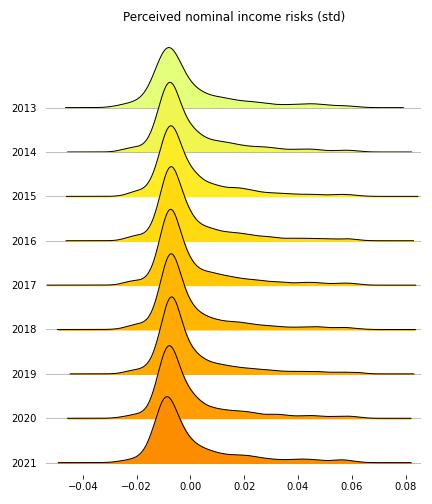
\includegraphics[width=0.4\textwidth]{figures/joy_incstd.jpg}
	\end{figure}
	\begin{itemize}
		\item  residuals controlling for observables /time fixed effects
		\item average PR:  $2.1\%$ in std; 10/90 IQR: $3.2\%$ in std \quad \hyperlink{rincstd_hist}{\beamerbutton{Back}}    
		% \item just a lower bound: before adjustment of unemployment risk 
	\end{itemize}
\end{frame}

\begin{frame}{Appendix: expected growth by age}
	\begin{figure}[ht]
		%\caption{Perceived Risk} 
		\label{appendix:age_gender_educ_level_compare_figure}
		\centering
		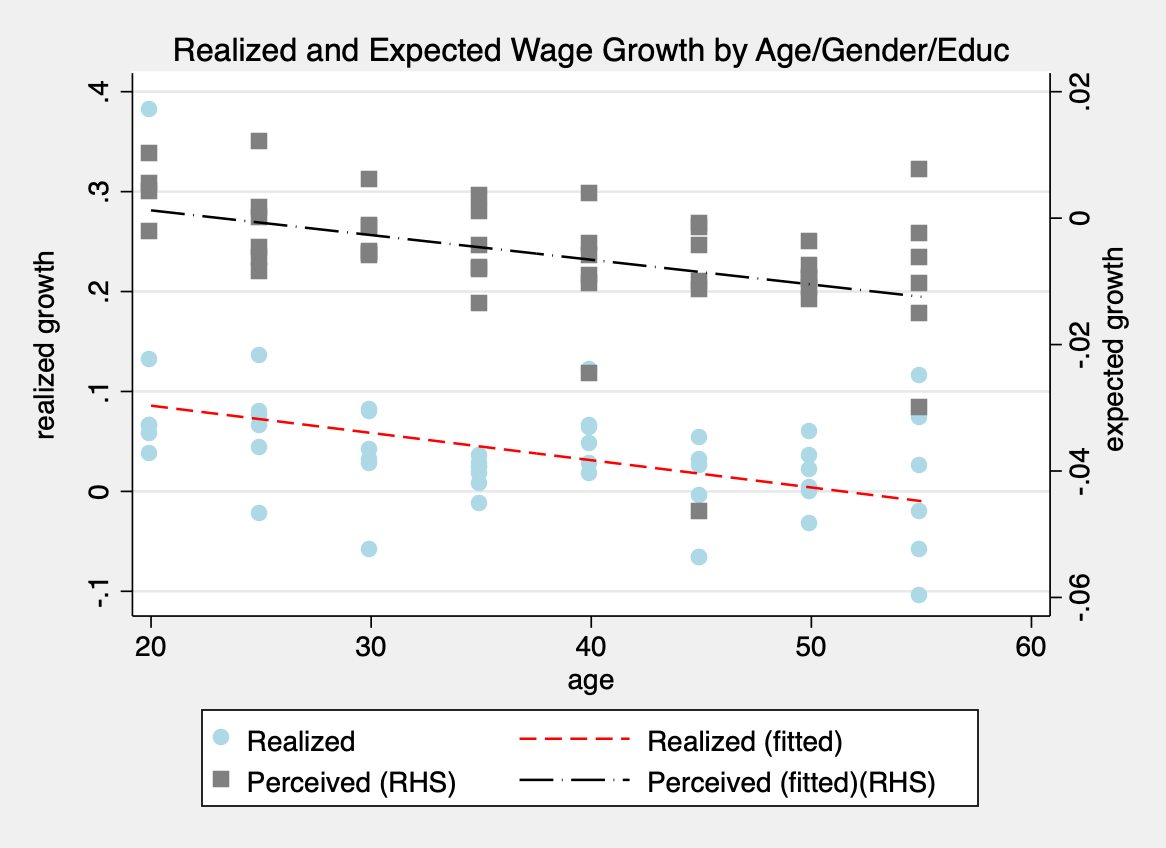
\includegraphics[width=0.7\textwidth]{figures/real_log_wage_gr_level_by_age_edu_gender_compare.png}
	\end{figure}
	\begin{itemize}
		\item e.g. a male high school graduate aged 30 
	\end{itemize}
\end{frame}


\begin{frame}{Appendix: expected \textbf{nominal} growth by age}
	\begin{figure}[ht]
		%\caption{Perceived Risk} 
		\label{appendix:age_gender_educ_nlevel_compare_figure}
		\centering
		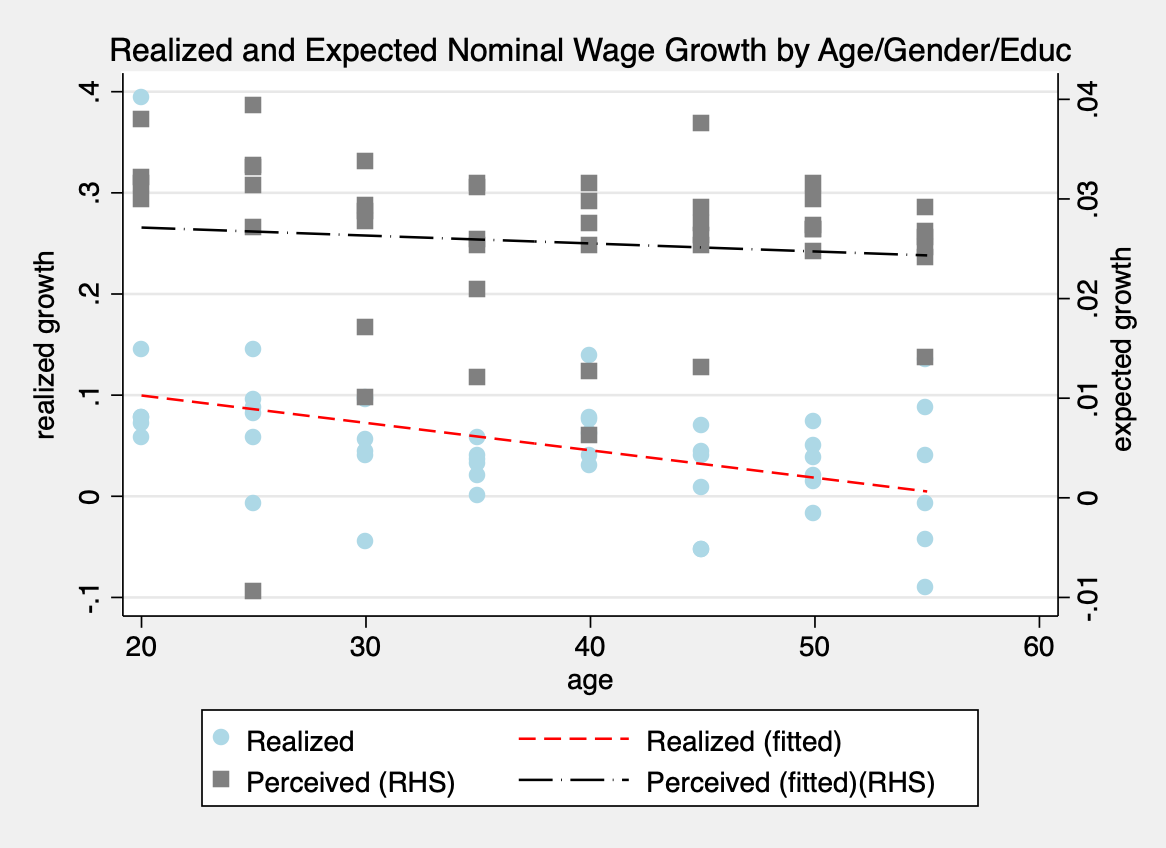
\includegraphics[width=0.7\textwidth]{figures/real_log_wage_gr_nlevel_by_age_edu_gender_compare.png}
	\end{figure}
	\begin{itemize}
		\item e.g. a male high school graduate aged 30 
	\end{itemize}
\end{frame}


%% since income risks may difer over time or stochastic,  so the level of risks are not comparable directly between two non-overlapping periods. % therefore, we can treat the income volatility in the past as experiences and examine if it affects risk perceptions. Here we differ from the earlier exercise in that we do not assume the risks are cohort specific. Instead, we just assume the information set, namely the experienced volatility and inequality are different.

% we find the experienced volatility is not correlated with risk perceptions over the past. But experienced inequality is positively correlated with the risk perceptions. 
% furthermore, the average economy has negative impacts on the risk perceptions as well. 


\begin{frame}{Appendix: Experienced volatility and PR}
	\label{appendix:experience}
	\begin{figure}
		\centering 
		\label{experience_var_var_var}
		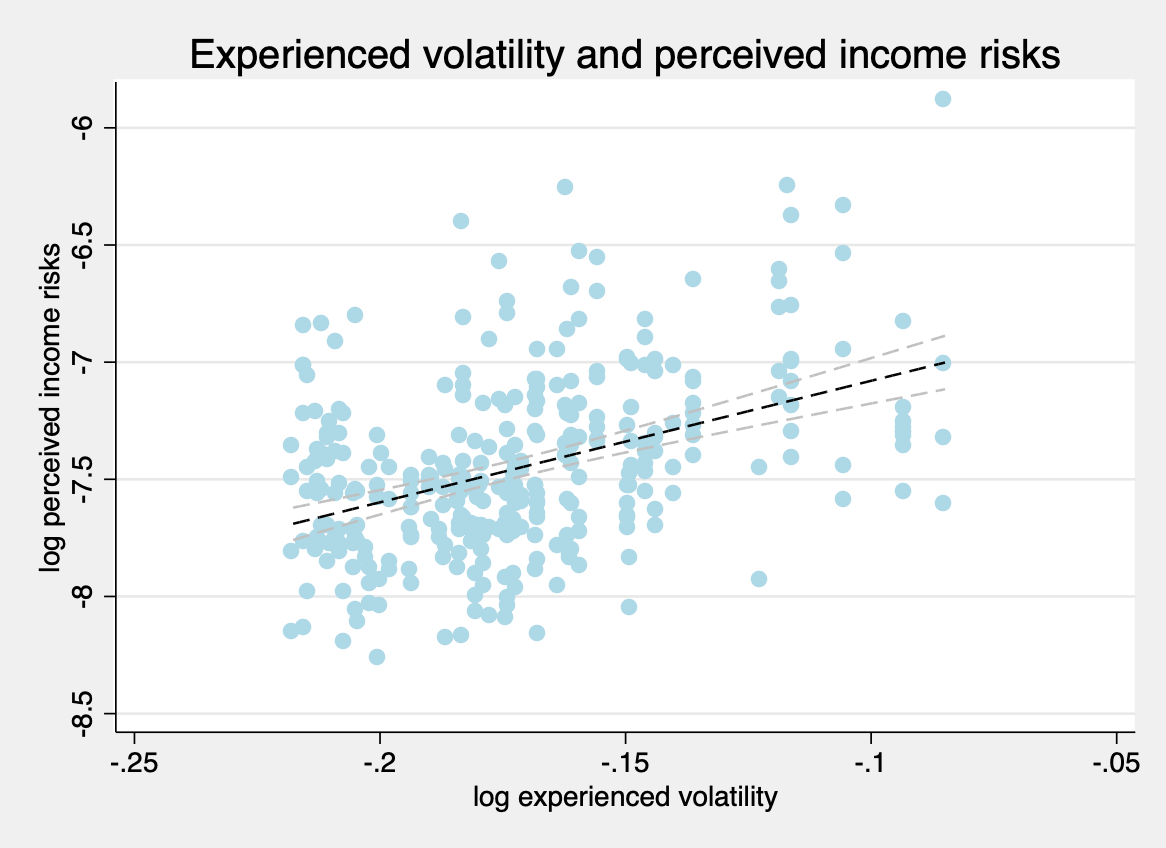
\includegraphics[width=0.6\textwidth]{figures/experience_var_var_data.png}
	\end{figure}
	\begin{itemize}
		\item income volatility conditional on macroeconomic history \cite{storesletten2004cyclical}
		\item e.g. the experience by a 25-year old till 2015 is between 1990-2015
	\end{itemize}
\end{frame}

\begin{frame}{Experienced labor market and perceived risks}
	\begin{figure}
		\centering 
		\label{experience_ue_var}
		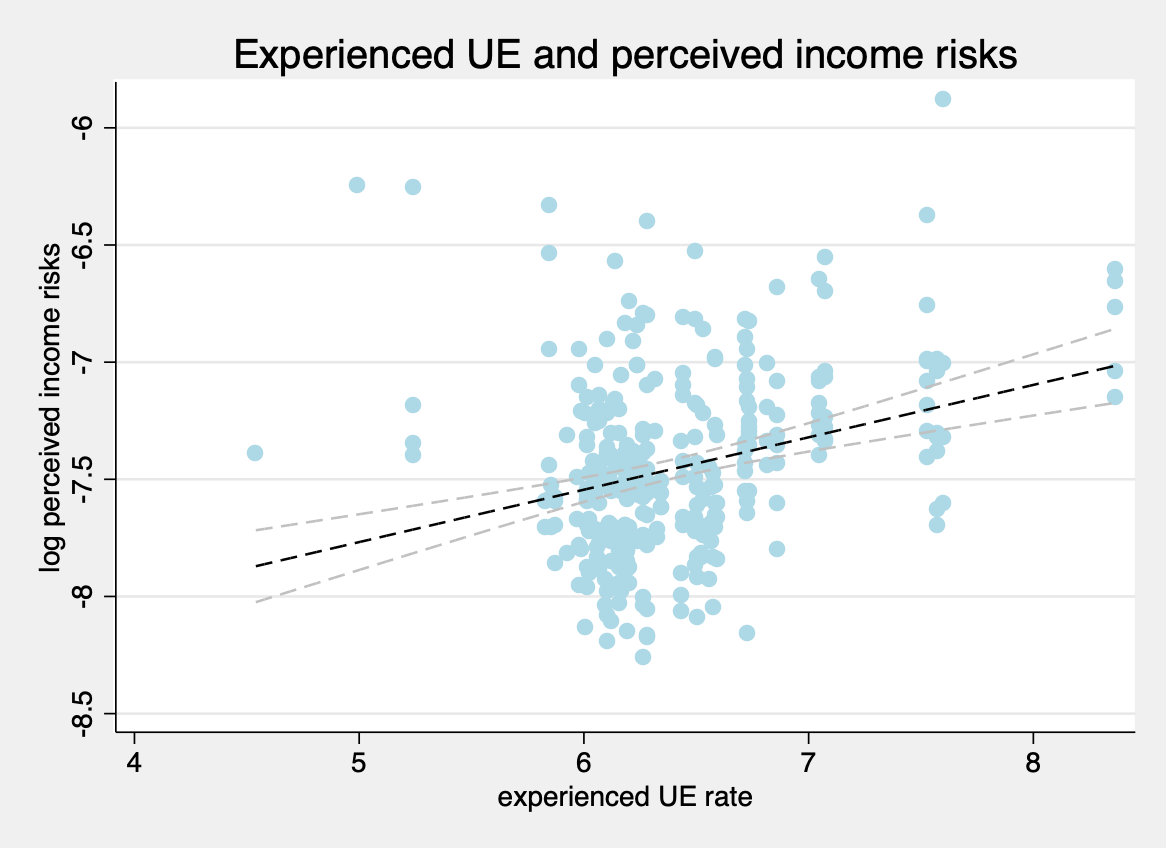
\includegraphics[width=0.6\textwidth]{figures/experience_ue_var_data.png}
	\end{figure}
	\begin{itemize}
		\item e.g. experienced UE by a 25-year old in 2015 is between UE over 1990-2015
		
	\end{itemize}
\end{frame}



\begin{frame}{Appendix: Extrapolation from \textcolor{blue}{individual} experiences}
	\label{appendix:extrapolation}
	\begin{itemize}
		\item higher experienced volatility $\rightarrow$ higher PR
		\item recent unemployment experience $\rightarrow$ higher PR
	\end{itemize}
	\begin{table}
		\centering
		\label{extrapolation}
		\adjustbox{max height=0.5\textheight, max width=\textwidth}{ 
			\begin{tabular}{lllllllllll}
				\hline 
				& (1)       & (2)       & (3)       & (4)       & (5)        & (6)        & (7)        & (8)        & (9)        & (10)       \\
				\hline 
				income shock squared                  & 0.0225*** & 0.0222*** & 0.0217*** & 0.0207*** & 0.000773   & 0.00205*** & 0.000566   & 0.00183*** & 0.000614   & 0.00184*** \\
				& (0.00562) & (0.00570) & (0.00562) & (0.00564) & (0.000743) & (0.000516) & (0.000744) & (0.000515) & (0.000745) & (0.000516) \\
				&           &           &           &           &            &            &            &            &            &            \\
				recently unemployed                   &           &           &           & 0.511*    & 0.228***   & 0.0895***  &            &            &            &            \\
				&           &           &           & (0.260)   & (0.0330)   & (0.0200)   &            &            &            &            \\
				&           &           &           &           &            &            &            &            &            &            \\
				unemployed since m-8&           &           &           &           &            &            & 0.161***   & 0.0783***  &            &            \\
				&           &           &           &           &            &            & (0.0207)   & (0.0121)   &            &            \\
				&           &           &           &           &            &            &            &            &            &            \\
				unemployed since y-1&           &           &           &           &            &            &            &            & 0.138***   & 0.0701***  \\
				&           &           &           &           &            &            &            &            & (0.0193)   & (0.0113)   \\
				Observations                          & 3662      & 3662      & 3662      & 3662      & 3701       & 1871       & 3701       & 1871       & 3701       & 1871       \\
				R-squared                             & 0.004     & 0.013     & 0.016     & 0.017     & 0.015      & 0.030      & 0.019      & 0.041      & 0.016      & 0.039      \\
				\hline 
			\end{tabular}
		}
	\end{table}
\end{frame}



\begin{frame}{Appendix: expected income growth and recent (past) wage growth}
	\label{appendix:tsMean3mvrexp_he}
	\begin{itemize}
		\item $\overline{\text{exp}_{t}} $: average expected growth across individuals
		\item  quarterly growth in average hourly wage
	\end{itemize}
	\begin{figure}
		\centering
		\label{ts_exp}
		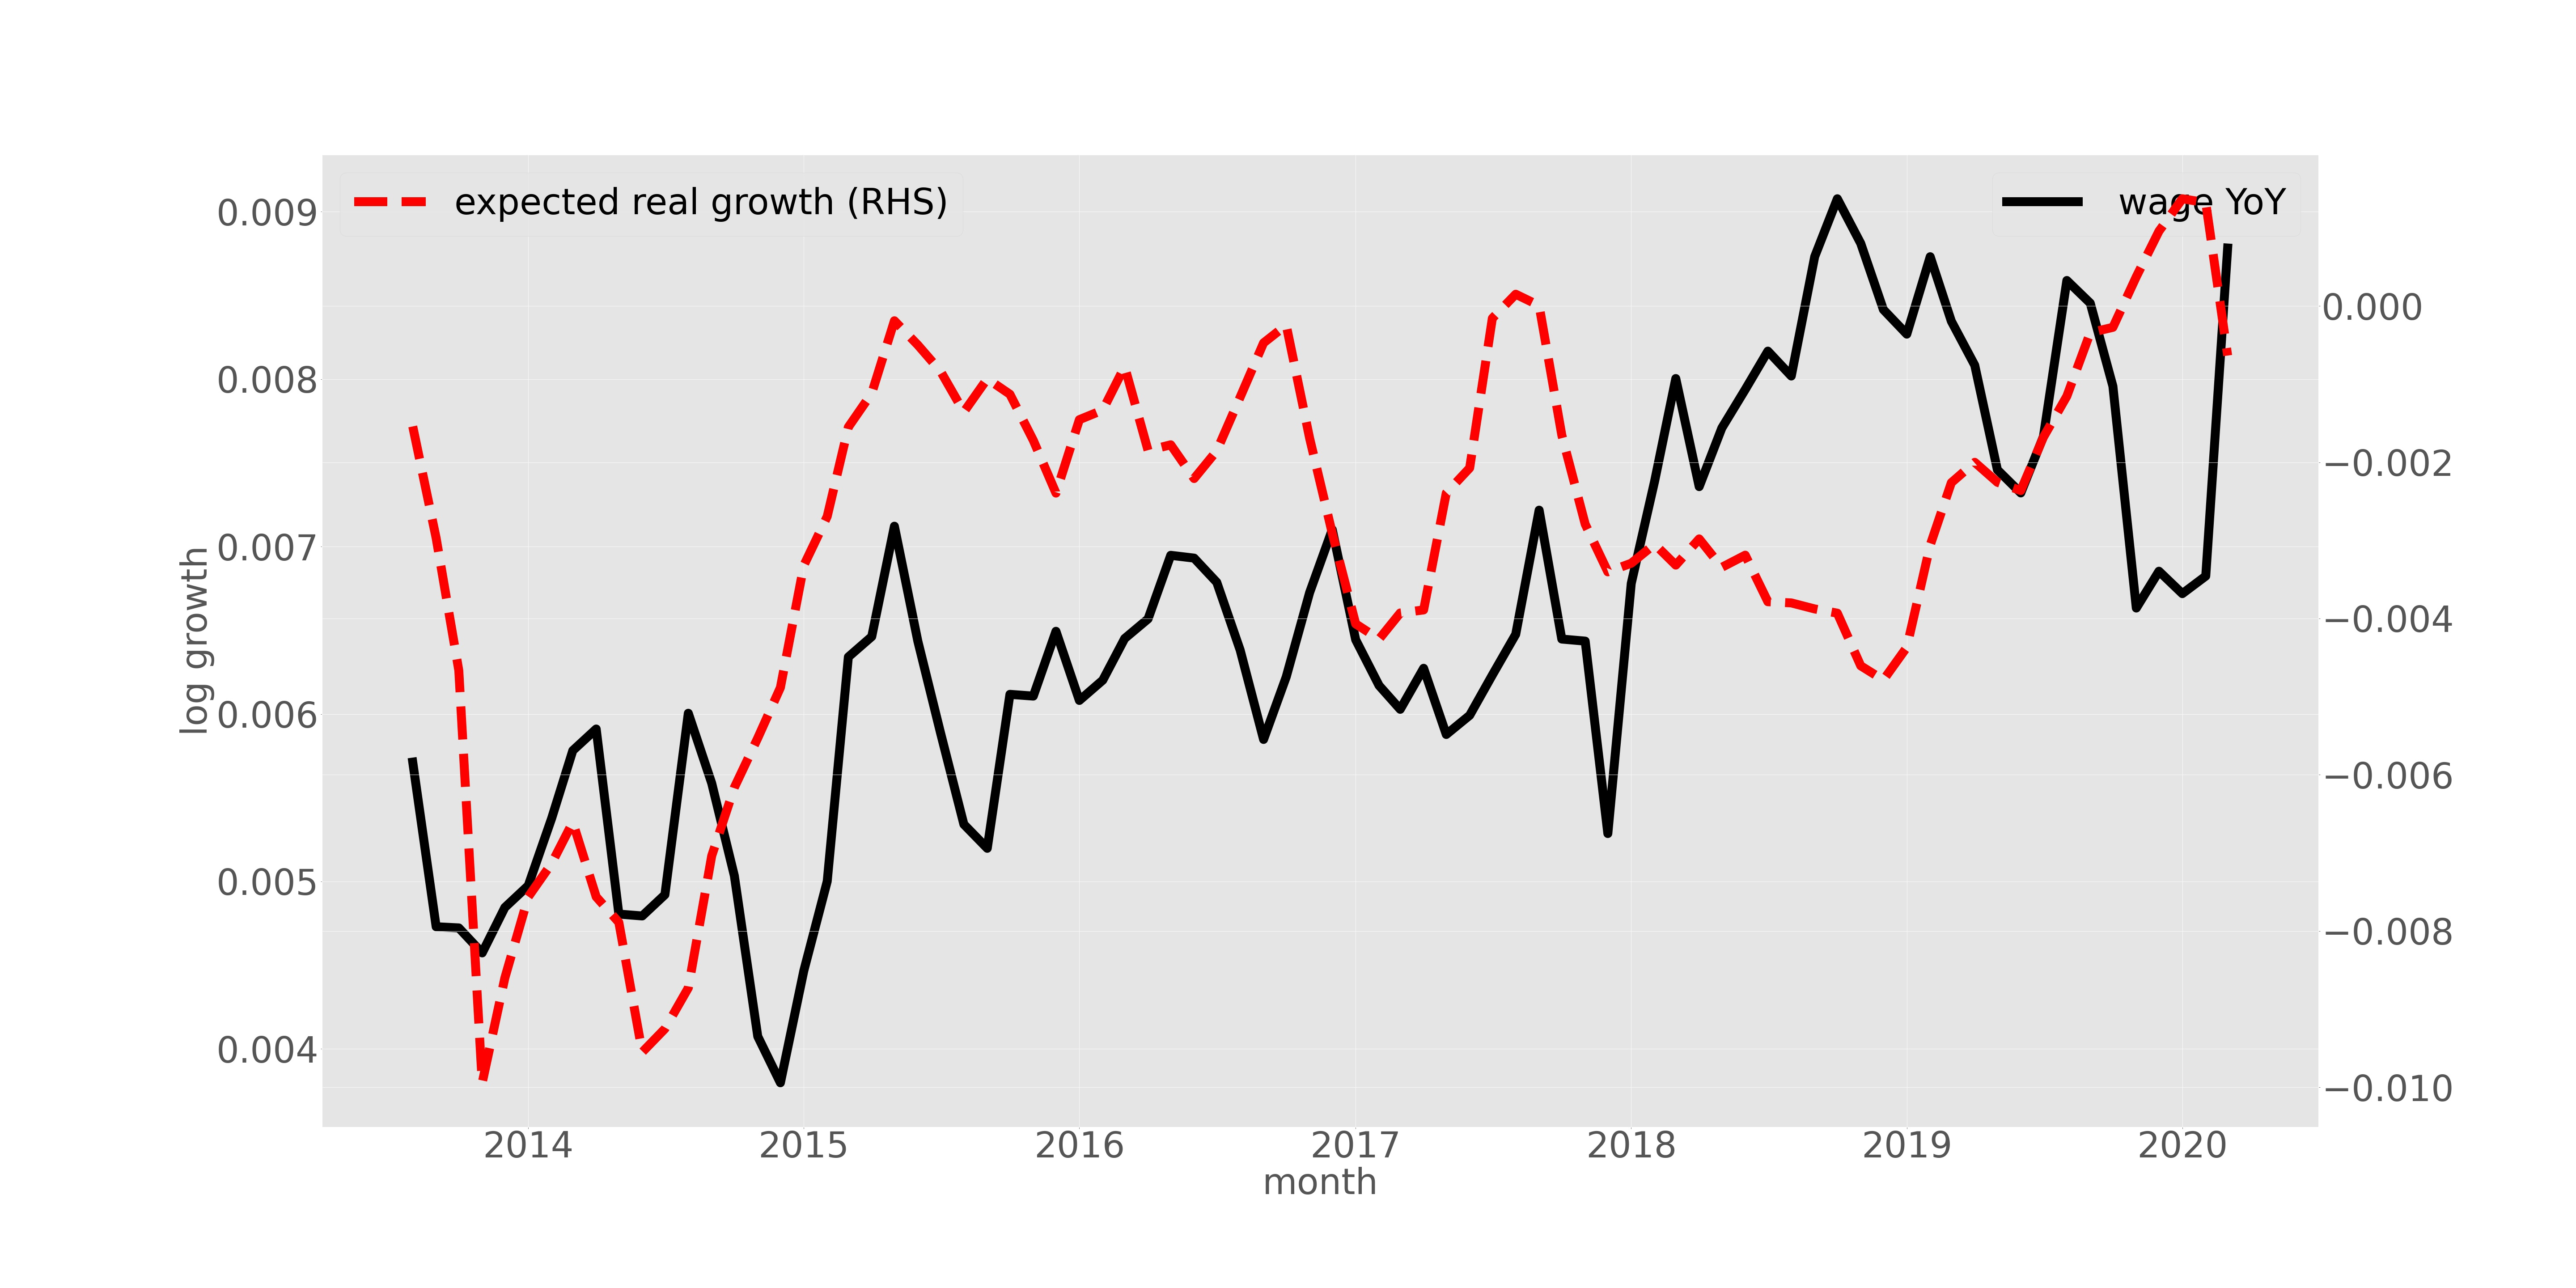
\includegraphics[width=0.9\textwidth]{figures/tsMean3mvrexp_he.jpg}
	\end{figure}
	\quad  \hyperlink{tsMean3mvrvar_he}{\beamerbutton{Back}} 
\end{frame}




\begin{frame}{Appendix: PR and current labor market condition}
		\label{appendix:PR_macro_labor_market_correlation}
	\begin{eqnarray*}
		\underbrace{\overline{\text{risk}_{t}}}_{\text{average perceived risk}} = \alpha + \textcolor{red}{\beta} \underbrace{(log(\text{wage}_{t-k/12}) - log(\text{wage}_{t-(k-3)/12}))}  _{\text{wage growth}}  + \epsilon_{i,t}	 \\
		\quad \forall k =0...4
	\end{eqnarray*}
	
	\begin{table}
		\centering
		%\caption{Correlation between Perceived Income Risks and Stock Market Return}
		\label{macro_corr_he}
		\adjustbox{max height=0.5\textheight, max width=\textwidth}{ 
			\begin{tabular}{lllll}
				\hline 
				& mean:var & mean:iqr & mean:rvar & mean:skew \\
				\hline 
				0 & -0.28**  & -0.42*** & -0.48***  & -0.02     \\
				1 & -0.42*** & -0.53*** & -0.51***  & 0.12      \\
				2 & -0.43*** & -0.48*** & -0.44***  & -0.01     \\
				3 & -0.43*** & -0.48*** & -0.42***  & -0.1      \\
				4 & -0.31*** & -0.41*** & -0.32***  & -0.21*   \\
				\hline 
			\end{tabular}
		}
	\end{table}
	\begin{itemize}
		\item Counter-cyclical income risks: \cite{storesletten2004cyclical}, \cite{guvenen2014nature}, \cite{bayer2019precautionary}
		%\item Counter-cyclical skewness: \cite{guvenen_empirical_2009}, \cite{guvenen_inferring_2014} 
	\end{itemize}
	\quad  \hyperlink{tsMean3mvrvar_he}{\beamerbutton{Back}} 
\end{frame}



\begin{frame}{Appendix: PR  and current labor market condition}
	\label{appendix:PR_state_labor_market}
	\begin{eqnarray*}
		\underbrace{\overline{\text{risk}_{s,t}} }_{\text{median perceived risk in state $s$}}= r + \textcolor{red}{\psi} \underbrace{LM_{s,t}}_{\text{state labor market condition}}  + \eta_{s,t}
	\end{eqnarray*}
	\begin{table}
		\centering
		%\caption{Correlation between Perceived Income Risks and Stock Market Return}
		\label{macro_corr_he_state}
		\adjustbox{max height=0.5\textheight, max width=\textwidth}{ 
			\begin{tabular}{lllll}
				\hline 
				& (1)                & (2)                & (3)               & (4)               \\
				\hline 
				& log(var) & log(risk) & log(iqr) & log(iqr) \\
				\hline 
				wage growth & -0.05***           &                    & -0.03***          &                   \\
				
				& (0.01)             &                    & (0.01)            &                   \\
				unemp rate &                    & 0.04*              &                   & 0.04***           \\
				&                    & (0.02)             &                   & (0.01)            \\
				\hline 
				Observations      & 3529               & 3529               & 3546              & 3546              \\
				R-squared         & 0.023              & 0.020              & 0.025             & 0.028            \\
				\hline 
			\end{tabular}
		}
	\end{table}
	\quad  \hyperlink{tsMean3mvrvar_he}{\beamerbutton{Back}} 
\end{frame}


\begin{frame}{Appendix: monthly earning inequality and volatility}
	\label{appendix:monthly_inequality_vol}
	\begin{figure}[ht]
	\centering
	\begin{subfigure}[b]{0.46\textwidth}
		\caption{Inequality}
		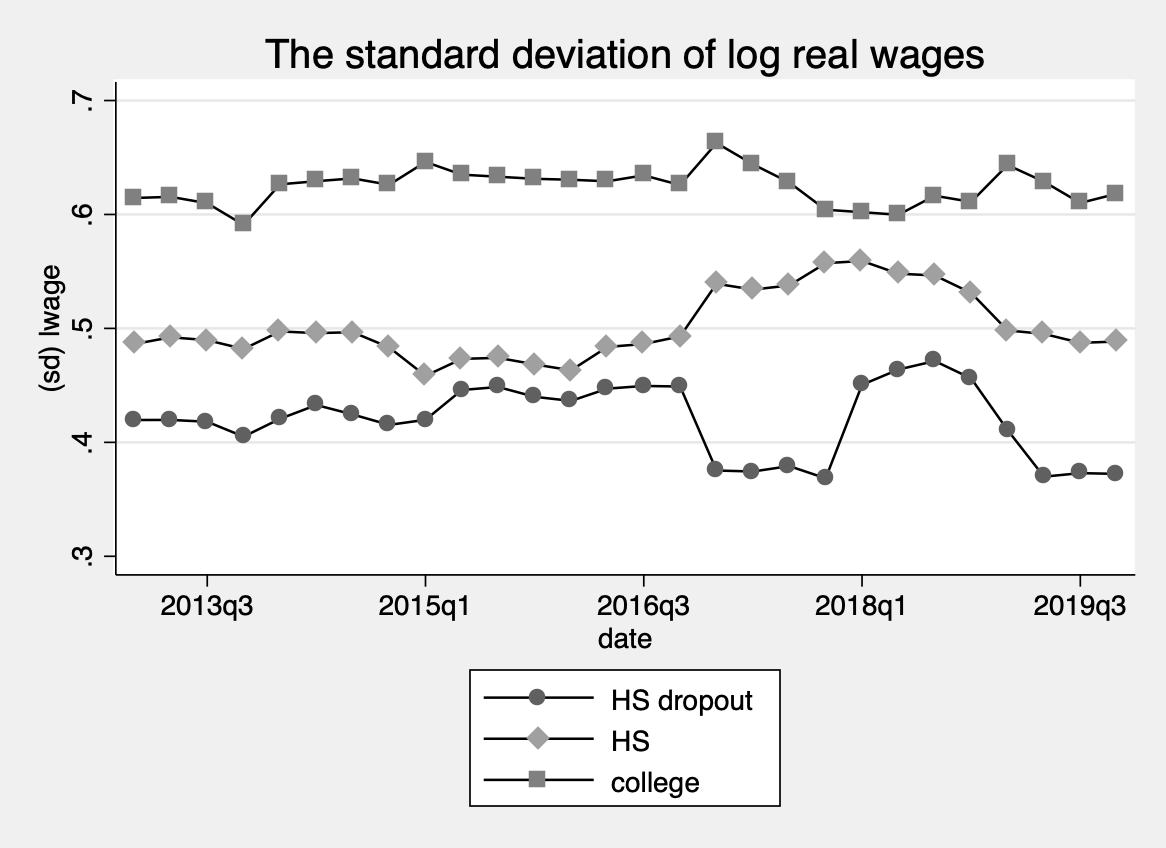
\includegraphics[width=\textwidth]{figures/log_wage_sd_by_edu.png}
	\end{subfigure}
	\begin{subfigure}[b]{0.46\textwidth}
		\caption{Volatility}
		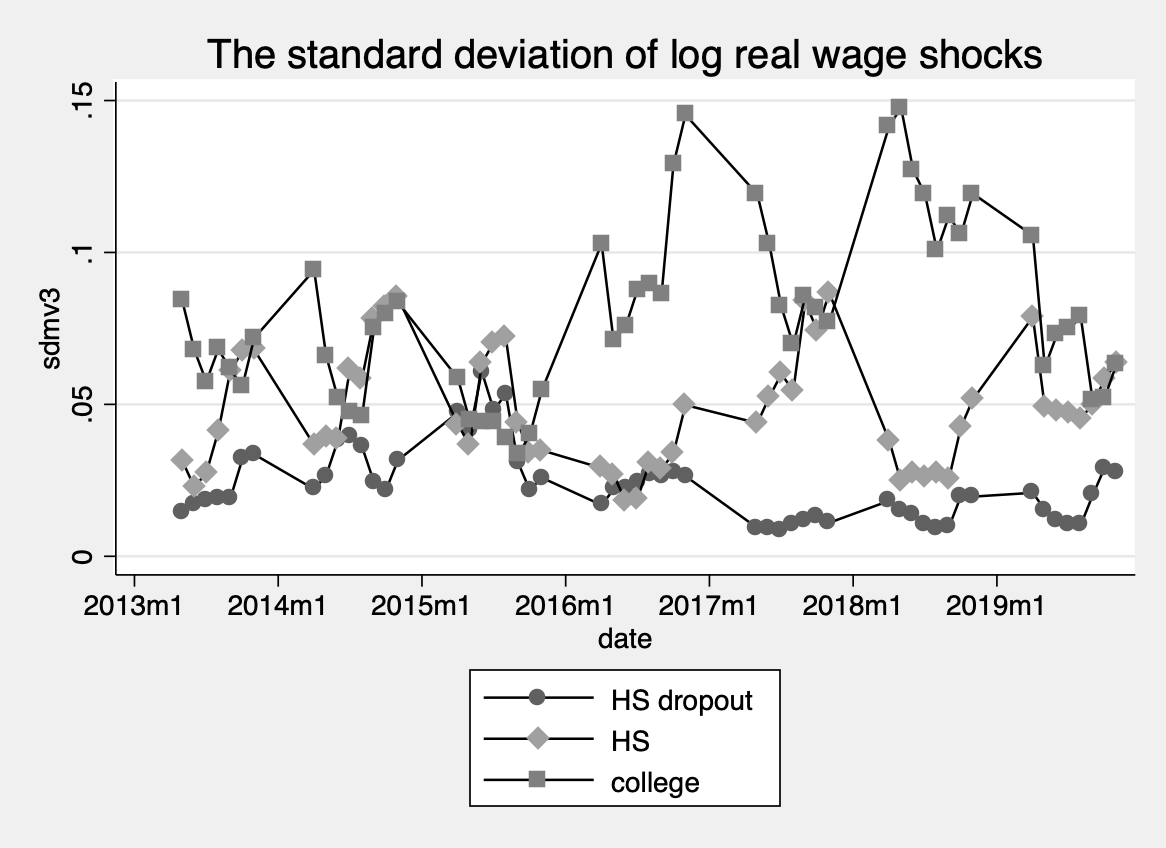
\includegraphics[width=\textwidth]{figures/log_wage_shk_gr_sd_by_edu.png}
	\end{subfigure} 
\end{figure}
	\hyperlink{monthly_decomposition_compare}{\beamerbutton{Back}} 
\end{frame}





\begin{frame}{Appendix: estimating state-dependent PR using survey}
	\label{RegimeEstimation}
	
	\begin{equation*}
		\begin{split}
			&	\underbrace{\tilde \Gamma^s_{i,t}}_{\text{reported PR}} = \underbrace{\tilde \Gamma_l + \mathbbm{1}(\overbrace{J_{i,t}}^{\text{Hidden state}}= 1)( \tilde \Gamma_h -\tilde \Gamma_l)}_{\tilde \Gamma_{i,t}} +\xi_{t}+\eta_{i}+ \epsilon_{i,t}\\
			& \text{Prob}(J_{i,t+1}|J_{i,t}) = \Omega
		\end{split}
	\end{equation*}
	
	%\begin{equation*}
	%	\begin{split}
		%		\log(\tilde {\text{var}}_{i,t})= (12+\frac{1}{12\kappa^2})\tilde \sigma^2_{i,t,\psi} + \xi_{t}+\eta_{i}+ \epsilon_{i,t}
		%	\end{split}
	%\end{equation*}
	\begin{itemize}
		
		\item $J_{i,t} =0$ for low and $=1$ for high PR state
		\item a short time series of $\tilde \Gamma_ {i,t}$ for many $i$s observed in the survey 
		\item $\{\tilde \Gamma_l\,\tilde \Gamma_h,\Omega\}$ can be estimated by $MLE$
		%\item $\kappa$: externally assumed ratio of permanent and transitory risks $\frac{\tilde \sigma_{i,t,\psi}}{\tilde \sigma_{i,t,\theta}}$
		\item a modified \cite{hamilton1989new} 2-regime-switching model 
		\item $J_{i.t}$ can be also dependent upon business cycles 
	\end{itemize}
	\hyperlink{appendix:RegimeEstimationDetail}{\beamerbutton{More details}} 
\end{frame}


\begin{frame}{Appendix: estimating state-dependent PR using survey}
	\label{appendix:RegimeEstimationDetail}
	
	\begin{equation*}
		\begin{split}
				\log(\tilde {\text{var}}_{i,t})= (12+\frac{1}{12\kappa^2})\tilde \sigma^2_{i,t,\psi} + \xi_{t}+\eta_{i}+ \epsilon_{i,t}
			\end{split}
	\end{equation*}
	\begin{itemize}
		
		\item $\kappa$: externally assumed ratio of permanent and transitory risks $\frac{\tilde \sigma_{i,t,\psi}}{\tilde \sigma_{i,t,\theta}}$
		\end{itemize}
	\hyperlink{RegimeEstimation}{\beamerbutton{Back}} 
\end{frame}



\begin{comment}


\begin{frame}{Extensions: additional heterogeneity in $MPC$}
	
	\begin{itemize}
		\item Heterogeneous time preferences
		\begin{itemize}
			\item Ex-ante differences in $\beta$, a la \cite{krusell1998income,carroll2017distribution,krueger2016macroeconomics}.
		\end{itemize}
		\item Costly adjustments
		\begin{equation*}
			\begin{split}
				& V_{i,\tau}(c_{i,\tau-1},x_{i,\tau}) = \textrm{max} \quad \{V^A_{\tau}(x_{i,\tau})-\chi,V^N_{\tau}(c_{i,\tau-1},x_{i,\tau})\} \\
				& V^A_{\tau}(x_{i,\tau}) = \underset{\{c_{i,\tau}\}}{\textrm{max}} \quad u(c_{i,\tau}) + (1-D)\beta \mathbb{E}_{\tau}\left[V_{\tau+1}(x_{i,\tau+1})\right]  \\
				& V^N_{\tau}(c_{i,\tau-1},x_{i,\tau}) =  u(c_{i,\tau-1}) + (1-D)\beta \mathbb{E}_{\tau}\left[V_{\tau+1}(c_{i,\tau},x_{i,\tau+1})\right]
			\end{split}
		\end{equation*}
		\begin{itemize}
			\item Utility cost from adjusting consumption in each period
			\item To introduce extensive margin of consumption change and match high $MPC$ from data 
		\end{itemize}
	\end{itemize}
\end{frame}

\end{comment}

\bibliographystyle{apalike}
\bibliography{PIR_slides}


\end{document}
